%% This work is licensed under the Creative Commons Attribution-NonCommercial-NoDerivs 3.0 Unported License.
%% To view a copy of this license, visit www.creative-commons.org/licenses/by-nc-nd/3.0 or send a letter
%% to Creative Commons, 444 Cas-tro Street, Suite 900, Mountain View, California, 94041, USA.

%% The above statement applies to all included files too!!!

\documentclass[a4paper,12pt]{article}

\usepackage[
	%iwona,
	%final,
	blacklogo,
	%joinlists,
	abbreviations,
	figures,
	tables,
	listings,
	language=czech,
	bibfile=bibliography.bib,
	bibencoding=utf8,
	bibstyle=numeric,
	encoding=utf8,
	]{upbase}

\usepackage[
	custompicture=graphics/elephant.png
	]{upsimple}
	
\usepackage{caption}
\usepackage[list=true]{subcaption}
\usepackage[shortcuts]{extdash}

\uptitle{Databázové systémy 1}
\upsubtitle{KMI/DATA1}
\upyear{\today}
\upauthor{Martin Rotter}
\upanot{Tento dokument obsahuje přepisy přednášek, které vedl \href{mailto:vilem.vychodil@upol.cz}{doc. RNDr Vilém Vychodil, Ph.D.}. Uvedená práce (dílo) podléhá licenci \href{http://creativecommons.org/licenses/by-nc-nd/3.0/}{Attribution-NonCommercial-NoDerivs 3.0 Unported}, a to včetně vložených souborů, to neplatí pro loga jiných společností, jako je například logo \href{http://www.postgresql.org/}{PostgreSQL}.}
\uppapertype{P\v{R}EPISY P\v{R}EDN\'{A}\v{S}EK}

\DeclareMathOperator{\dom}{dom}
\DeclareMathOperator{\typ}{typ}
\DeclareMathOperator{\degree}{degree}
\DeclareMathOperator{\Mod}{Mod}
\begin{document}

% vytiskne titulní stranu
\upmaketitle

% vytiskne anotaci (abstrakt)
\upmakeanot

% tiskne obsah a seznamy obrázku, tabulek a případně zdr. kódů, více v makrech \uptableofcontents a \upprintlists
% tiskne pouze povolené seznamy
\uptocandlists

% deklarace zkratek
\upabbrevdeclare{DBMS}{DBMS}{Database Management System}
\upabbrevdeclare{SQL}{SQL}{Structured Query Language}
\upabbrevdeclare{RA}{RA}{Relační algebra}
\upabbrevdeclare{BCNF}{BCNF}{Boyce--Codova normální forma}
\upabbrevdeclare{3NF}{3NF}{3. normální forma}
\upabbrevdeclare{2NF}{2NF}{2. normální forma}
\upabbrevdeclare{1NF}{1NF}{1. normální forma}

% první přednáška
\section{Přehled databázových systémů a jejich historie}

Databázový systém (anglicky \upabbrevref{DBMS}) je soustava komplexního aplikačního vybavení, které je podloženo určitým teoretickým základem. Jeden bez druhého nemůže existovat (resp. může, což má ale za následek formální selhání \upabbrevref{DBMS} jako takového), a tak je nutné znát obě strany pomyslné databázové barikády. Databázový systém tedy tvoří:
\begin{enumerate}
\item Aplikační software, který je obvykle používán jako rozhraní pro přístup k databázi samotné.
\item Teorie, která formálně podkládá návrh databáze, organizaci dat a obsahuje algoritmickou stránku věci.
\end{enumerate}

Mějme na paměti, že obě části databázových systémů se rozvíjely postupně a mnohdy metodou pokus - omyl. Obecně platí, že pokud selže teoretický základ, tak již ani sebelepší frontend nic nezmůže. V databázovém systému se objeví formální rozpor a jedinou cestou vpřed je začít znovu.

Hlavním úkolem \upabbrevref{DBMS} je poskytovat \textit{perzistentní uložení dat}, dále poskytnout svým uživatelům konzistentní rozhraní a případně nabídnout \textit{transa\-kční zpracování dat}. Nutnto podotknout, že poslední bod nemusí být takovou samozřejmostí, jak by se mohlo zdát.

\subsection{Historie databázových systémů}
Potřeba organizace dat je stará jako lidstvo samo. Již staří Egypťané si vedli podrobné záznamy o výběru daní, stavbách chrámů a jiných činnostech. Zde můžeme hovořit o databázích založených na souborech.

\subsubsection{Databáze založené na souborech}
Souborem může být například papyrus, hliněná destička nebo (lépe) papír. Na papíře mohou být napsány v řádcích nějaké záznamy. Například seznam dlužníků nějakého podnikatele. \textit{Vytvoření} takového seznamu je vskutku \textit{lehké}. Představme si, že dlužník uprostřed seznamu splatil svůj dluh a bude ze seznamu vyškrtnut. Místo něj v seznamu vznikne prázdné místo. Zbytek seznamu se následně musí zkonsolidovat (přepsat na nový papír), aby vypadal konzistentně. Odtud plyne určitá \textit{těžkopádnost} vyplývající z definice souboru a z určité \textit{nízkoúrovňovosti} práce s ním. Přitom souborem může být myšlen i soubor na disku počítače.

Představme si navíc, že daný podnikatel si vede další soubor se seznamem, kde si u každého dlužníka značí jeho adresu, aby jej mohl v případě nutnosti navštívit. Jméno dlužníka tedy uchováva hned na dvou seznamech, přitom je přirozeně jasné, že stačí dlužníka evidovat jednou a poté se na něj \enquote{odkazovat.} \textit{Redundace dat} je tedy zřejmá.

\subsubsection{Databáze založené na síťovém modelu}
Průkopníkem této oblasti byl Charles Bachman. Aktuálně se toto paradigma považuje za dávno překonané, nicméně pro časy budoucí poskytlo několik dob-rých poznatků. Typicky \enquote{síťový} databázový systém je tvořen mj. i:
\begin{enumerate}
\item \textit{Záznamy}, které mají určitý \textit{typ}. Ten deklaruje, jaké \textit{atributy} daný záznam obsahuje. Atributy mohou nabývat různých hodnot.
\item \textit{Odkazy}, které reprezentují \textit{vztahy} mezi jednotlivými záznamy.
\end{enumerate}
Obecně se ví, že databázové systémy tohoto typu mohou poskytovat velmi rychlé prostředky pro získávání jednoduchých dat, ale na druhou stranu na komplexnější data se dotazuje hůře. Tvorba dat není rovněž jednoduchá, protože práce s odkazy požaduje vyšší míru sofistikace.

\begin{figure}
\centering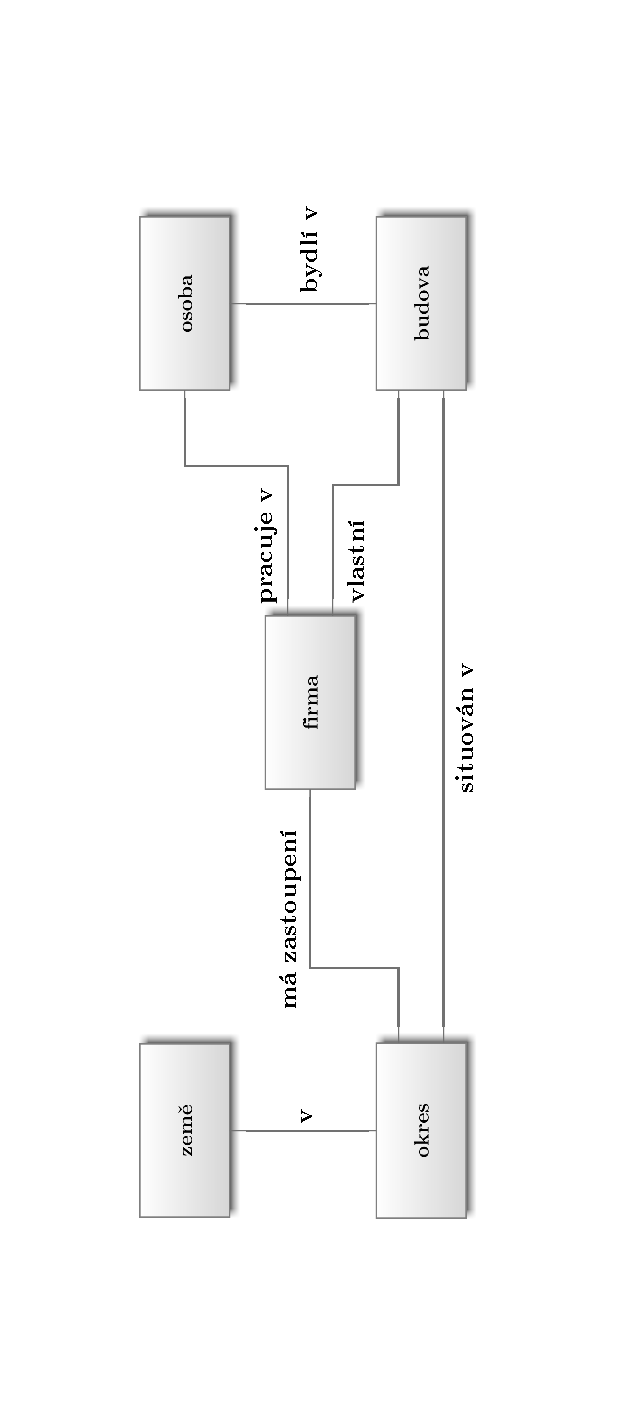
\includegraphics[angle=-90,width=14cm]{graphics/01-sitovy}
\caption{Datový model s obousměrnými odkazy}
\end{figure}

\begin{figure}
\centering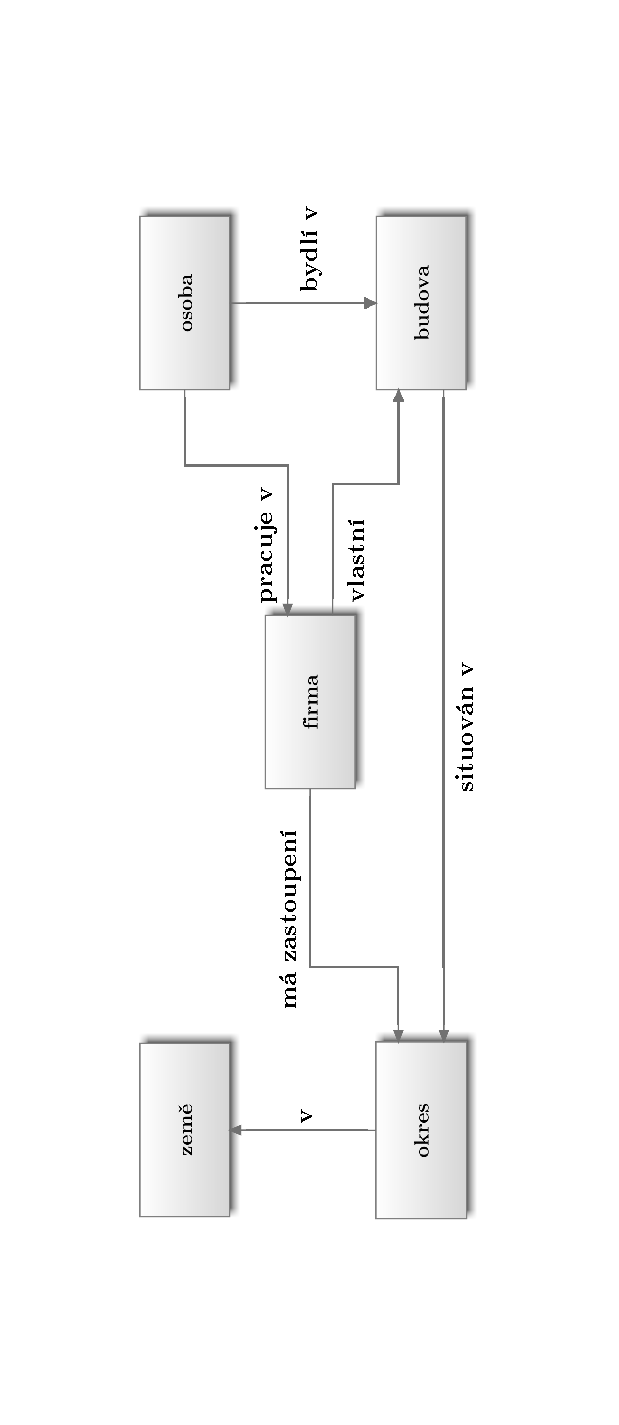
\includegraphics[angle=-90,width=14cm]{graphics/01-sitovy2}
\caption{Datový model s jednosměrnými odkazy}
\end{figure}

\subsubsection{Databáze založené na hierarchickém modelu}
Jedná se o speciální typ síťového modelu, kde bylo úmyslem tento model zjednodušit. Výsledkem bylo vytvoření hierarchie v záznamech a odkazech ve formě stromu\footnote{Strom je jednou ze základních grafových struktur. Jedná se o (neorientovaný) graf bez kružnic. Více napoví \citep[str. 91 -- 96]{cormen:algorithms}.}.

\subsubsection{Databáze založené na objektovém modelu}
V objektovém modelu jsou hlavní prvky, jež reprezentují data, \textit{objekty}, tedy serializované entity, které lze interpretovat pomocí nějakého vyššího programovacího jazyka. Prvním jazykem podporujícím takovéto pojetí byl Common Lisp.

\subsubsection{Databáze založené na relačním modelu}
Jedná se o aktuálně používaný model, který přináší určité výhody. Primárním nosičem informace v tomto modelu jsou \textit{relace} (poněkud amatérsky je můžeme nazývat také tabulkami). Základy tohoto modelu položil Edgar Codd v roce 1970.\citep{codd:relationalModel}

\subsubsection{Nerelační databáze}
Vyvíjeny v 90. letech 20. století. Někdy chybně značovaný jako \uv{No SQL}. Rychlé pro jednoduché dotazy. Patří sem např. BerkeleyDB, MongoDB.
% obrázek struktury databáze.

\section{Relační model dat}
Model má 3 základní komponenty:
\begin{enumerate}
\item \textit{Struktury}, které uchovávají data a reprezentují výsledky dotazů.
\item \textit{Integritní omezení}, která popisují vztahy mezi daty, které musí být splněny. Integritní omezení jsou v podstatě formule. Tato omezení slouží k popisu toho, jak mají data vypadat, slouží k odstranění jejich chyb.
\item \textit{Manipulativní formalismy}, které říkají jak z uložených dat získat jiná data určitými operacemi.
\end{enumerate}
Relační model je konkrétním modelem dat, avšak modely jako takové lze rozdělit do dvou skupin, tedy:
\begin{enumerate}
\item Abstraktní modely dat, které poskytují vyčerpávající logické definice datových struktur nebo operací s daty. Ty dohromady tvoří abstraktní formalismus. Tedy jakýsi abstraktní stroj, se kterým může uživatel operovat.
\item Konkrétní implementace modelů, pracující s persistentními daty. Od uživa\-/tele databáze se očekává dobrá znalost modelu dat, detailní znalost fyzické implementace není nutná.
\end{enumerate}

\section{Struktura relačních dat}
Základním kamenem dat jsou tzv. \enquote{datové tabulky}, které obsahují záhlaví a další data.
\begin{enumerate}
\item Záhlaví (viz. tabulka \ref{tab:zahlavi}) je množina atributů a jejich typů. U tabulky se seznamem zamě\-stnanců může být atributem například jméno zaměstnance, rodné číslo atp.
\item Vlastní data (neboli tělo) tabulky by u takovéto tabulky představovala data samotných zaměstnanců.
\end{enumerate}

\begin{table}
\caption{Záhlaví tabulky}\label{tab:zahlavi}
\begin{center}
\begin{tabular}{|c|c|c|}
\hline
ID & JMÉNO & ADRESA \\
\hline
15 & Vyacheslav Drsoň & Peklo, 666 \\
\hline
\vdots & \vdots & \vdots \\
\hline
\end{tabular}
\end{center}
\end{table}

\subsection{Požadavky na tabulky}
\begin{enumerate}
\item\label{enum:first_re} Řádky by neměly mít žádné pořadí. Tabulka by měla být chápána jako množina řádků. A v množině na pořadí nezáleží.
\item To samé platí pro sloupce.
\item Z definice množiny také vyplývá, že tabulka by neměla obsahovat identické řádky. Tento požadavek není v mnoha \upabbrevref{DBMS} splněn.
\item V každém poli uvnitř tabulky je právě jedna hodnota daného typu.(SQL porušuje nedefinovanou hodnotou)
\item\label{enum:last_re} Všechny atributy jsou regulární.(Nejsou přítomné žádné skryté atributy.)
\end{enumerate}
Tyto požadavky formuloval C.~J.~Date.
Pokud tabulka splňuje body \ref{enum:first_re} až \ref{enum:last_re}, pak je v 1. normální formě.

Zavedli jsme si několik pojmů jako \textit{atribut} a tak dále. Formalizujme je nyní přesněji:
\begin{description}
\item[Atribut] popisuje účel daného sloupce v tabulce, je to jméno sloupce.
\item[Typ] je jméno(označení) datového typu. Např.: INTEGER
\item[Doména] je množinou všech možných hodnot daného typu. Tedy například nějaký pomyslný typ\upinlinecode{SQL}{!}{BOOL} by mohl mít doménu ve tvaru: $$
\dom(BOOL) = \left\{ true, false \right\}
$$
\end{description}

\subsection{Relační schéma}
Již dříve jsme si uvedli pojem \textit{záhlaví tabulky}, avšak ten byl poněkud vágní. Relační schéma je jeho analogií s přesnější definicí.
\begin{uptheorem}[Relační schéma]
Mějme spočetnou množinu atributů $Y$ a mno\-/žinu typů $T$ Následně platí, relační schéma $R$ je množina definovaná jako:
$$
R = \left\{ \left\langle y, t \right\rangle \; | \; y \in Y, t \in T \right\}
$$
\end{uptheorem}
Proveďme dohodu, že typ atributu $y$ budeme zapisovat také jako $\typ(y)$ a analogicky doménu pro každý typ budeme značit jako $\dom(y)$.

\subsection{Obecné kartézské součiny}
Mějme následující systém množin:
$$
\left\{ A_{i} \; | \; i \in I \right\}
$$
kde $I$ je tzv. indexní (a libovolná) množina a $i$ je index z této množiny. Kartézský součin $A_{i} (i \in I)$ se značí $\prod_{i \in I} A_{i}$ a je definován jako množina všech zobrazení $$f: I \rightarrow \bigcup_{i \in I} A_{i} \text{ , kde } f(i) \in A_{i} \text{ pro } \forall i \in I$$.

Prvky $\prod_{i \in I} A_{i}$ jsou zobrazení, nezáleží v nich na pořadí indexů.
\begin{upexample}[Kartézský součin]
Vypočítejme kartézský součin množin $A$ a $B$, tedy $A \times B$ se zadáním:
$$
A = \left\{ a, b, c \right\}, \quad B = \left\{ 10, 20 \right\}, \quad I = \left\{ 1, 2 \right\}, \quad A_{1} = A, \quad A_{2} = B
$$
Následně řešení:
$$
\prod_{i \in \left\{ 1, 2 \right\}} A_{i} = \left\{ \left\langle a, 10 \right\rangle, \left\langle b, 10 \right\rangle, \left\langle c, 10 \right\rangle, \left\langle a, 20 \right\rangle, \left\langle b, 20 \right\rangle, \left\langle c, 20 \right\rangle \right\}\footnote{Zmíněnou rovnost nutno brát mírně s rezervou, protože formálně výsledkem kartézského součinu je množina zobrazení, nikoliv uspořádaných množin.}
$$
\end{upexample}

\begin{upexample}[Kartézský součin s tečkovou indexní množinou]
Mějme $I = \left\{ \bullet \right\}$ a $A_{\bullet}$. Pak platí, že $\prod_{i \in I} A_{\bullet} = A_{\bullet}$ s funkcí $f: \left\{ \bullet \right\} \rightarrow A_{\bullet}$.
\end{upexample}

\begin{upexample}[Kartézský součin žádné množiny]
Nechť $I = \varnothing$. Pak $\prod_{i \in I} A_{i} = \left\{ \varnothing \right\}$ s funkcí $f: \varnothing \rightarrow \varnothing$.
\end{upexample}

\subsection{Relace nad relačním schématem}
\begin{uptheorem}[Relace nad relačním schématem]
Mějme relační schéma $R\subseteq Y$, pak relace nad $R$ je libovolná konečná podmnožina kartézského součinu domén atributů z $R$, tedy
$$
\mathcal{D} \subseteq \prod_{y \in R} \dom(y)
$$
Relace v takovémto pojetí přibližně odpovídá vágnějšmu pojmu \textit{tabulka}. Součin lze pochopitelně také rozepsat. Obsahuje-li relační schéma $R$ celkem $n$ atributů, pak platí, že:
$$
\mathcal{D} \subseteq \dom(A_{1}) \times \cdots \times \dom(A_{n})
$$
Pozorný čtenář určitě pozoruje, že každá relace (tabulka) může mít určitý maximální možný počet řádků. Matematicky:
$$
\left|\mathcal{D}\right| = \left|dom(A_{1})\right| \times \cdots \times \left|dom(A_{n})\right|
$$
Relaci lze také označit jako dvojici $\left\langle \mathcal{D}, R \right\rangle$. Tato dvojice takřka kompletně popisuje tabulku.
\end{uptheorem}
Každý prvek relace (tabulky) se nazývá n-tice. To je analogické vzhledem k matematickému pojetí relaci jako takových. Matematické relace též obsahují n-tice.

\subsubsection{Speciální případy relací}
\begin{enumerate}
\item Prázdná relace (tabulka) nad $R$, tedy $\left\langle \varnothing, R \right\rangle$.
\item Tabulka \enquote{dum}, tedy $\left\langle \varnothing, \varnothing \right\rangle$.
\item Tabulka \enquote{dee}, tedy $\left\langle \left\{ \varnothing \right\}, \varnothing \right\rangle$.
\end{enumerate}

\section{Tutorial D}
Programovací jazyk Tutorial D formuje opozici vůči mnohem známějšímu a v praxi používanějšímu \upabbrevref{SQL}. Tutorial D má jedinou funkční a (víceménně) použitelnou implementaci známou jako Rel. Frontend Rel je naprogramován v jazyce Java a jeho prostředí vypadá bohužel hrůzostrašně. Rel je silně staticky typovaný, nemá konverze typů. Obsahuje typy:
\begin{description}
\item[Skalární], které jsou opozitem hodnotových typů ze známějších jazyků a patří sem například\upinlinecode{TutorialD}{!}{BOOLEAN},\upinlinecode{TutorialD}{!}{INTEGER} nebo\upinlinecode{TutorialD}{!}{CHARACTER} a také uživatelsky definované typy.
\item[N-ticové], které jsou dané jmény atributů a jejich typy.
\item[Relační], které jsou dány atributy a jejich typy. Hodnoty představují relace, t.j. množiny n-tic.
\end{description}


\subsection{Hodnoty vs. proměnné}
\begin{enumerate}
\item[Hodnoty] - jednotlivé konstanty, relace a n-tice. Nemohou se měnit, chovají se tedy \uv{jako ve Scheme}
\item[Proměnné] - ukazatele na reprezentace hodnot. Mají přiřazený typ, mohou měnit svůj odkaz.
\end{enumerate}

\subsection{Výrazy versus příkazy}
Výrazem v Tutorial D (resp. v Rel) je například prostá logická rovnost hodnot. Výraz může mít nějaký výsledek. Příkaz se od výrazu liší tak, že končí středníkem a obvykle obsahuje volání nějaké funkce.
\begin{upcode}{Výraz a příkaz (Tutorial D)}{}{TutorialD}
/* výraz */
666 = 6661215
/* příkaz */
WRITELN(10 = 20);
\end{upcode}

\subsection{N-tice jako hodnoty}
V Tutorial D lze přímočaře vytvářet řádky relací a považovat je za hodnoty, viz. kód \ref{code:valstuple}.
\begin{upcode}{Základy n-tic (Tutorial D)}{code:valstuple}{TutorialD}
/* prázdná n-tice */
TUPLE {}
/* n-tice včetně dat */
TUPLE {id 666, name "Vilík", lab 5077}
/* rovnost n-tic */
WRITELN(TUPLE {id 666, name "Vilík", lab 5077} = TUPLE {id 007, name "James Bond", lab 1111});
/* vnořené n-tice */
TUPLE {id 666, TUPLE {jmeno "Vilík" prijmeni "Devil"}, lab 5077}
\end{upcode}
Z n-tic lze pochopitelně získávat hodnoty nebo n-tice sjednocovat, zúžovat a tak podobně.
\begin{upcode}{Operace s n-ticemi (Tutorial D)}{}{TutorialD}
/* vypíše hodnoty atributů id a lab (zúžení n-tice) */
TUPLE {id 666, TUPLE {jmeno "Vilík" prijmeni "Devil"}, lab 5077} {id, lab}
/* vypíše vše kromě lab (zúžení n-tice) */
TUPLE {id 666, TUPLE {jmeno "Vilík" prijmeni "Devil"}, lab 5077} {ALL BUT lab}

/* sjednocení n-tic */
TUPLE {id 666, jmeno "Vilík"} UNION TUPLE {jmeno "Vilík", lab 5077}

/* přejmenování atributů n-tice */
TUPLE {id 666, jmeno "Vilík"} RENAME (id AS cislo, jmeno AS name)
\end{upcode}
Sjednocení n-tic bere dvě n-tice, které se shodují na nějakém atributu a ve výsledku se objeví konkatenace n-tic s jedním výskytem společného atributu. Kompozice n-tic funguje obdobně jako sjednocení, avšak ve výsledku se společné atributy vůbec neobjeví.
\begin{upcode}{Další operace s n-ticemi (Tutorial D)}{}{TutorialD}
/* rozšíření n-tice */
EXTEND TUPLE {id 666, jmeno "Vilík"} ADD (5077 AS lab)
/* aktualizace hodnot v n-tici */
UPDATE TUPLE {id 666, jmeno "Vilík"} (jmeno := "God")
\end{upcode}

\subsection{Relace v Tutorial D}
Tutorial D (potažmo Rel) samozřejmě podporuje relace.
\begin{upcode}{Operace s relacemi (Tutorial D)}{}{TutorialD}
/* relace s několika n-ticemi*/
RELATION {
	TUPLE {id 666, jmeno "Vilík"},
	TUPLE {id 007, jmeno "Bond"}
}
/* vytvoření relace jakožto typu */
VAR seznam_lidi BASE RELATION {id INTEGER, jmeno STRING} KEY {id};
\end{upcode}
% druhá přednáška
\section{Modifikace dat}
Již známe pojmy jako relace nebo relační proměnná. Modifikací dat v databázi se myslí přiřazení nové hodnoty k nějaké relační proměnné. V \upabbrevref{SQL} se k tomuto používají příkazy\upinlinecode{SQL}{!}{INSERT},\upinlinecode{SQL}{!}{UPDATE} nebo\upinlinecode{SQL}{!}{DELETE}. V Tutorial D k obdobným operacím slouží operátor \enquote{:=}, tak jak jej známe například z jazyka Pascal.
\begin{upcode}{Modifikace relace (SQL)}{}{SQL}
UPDATE	zakaznici
SET		plat = 0
WHERE	(plat > 50000);
\end{upcode}
\begin{upcode}{Modifikace relace (Tutorial D)}{}{Tutorial D}
INSERT zakaznici RELATION {TUPLE {id 666, jmeno "Vilík", }};
\end{upcode}
K získávání dat z databáze slouží tzv. \textit{relační dotazování}. Formátování dotazů pak definuje \textit{dotazovací jazyk}. Ten říká, jak se budou dotazy vyhodnocovat. Tyto jazyky jsou obvykle deklarativní. Známe například \upabbrevref{SQL} a Tutorial D.

\textit{Relační algebra} specifikuje množinu operací s relacemmi a dotazy se skládají z~postupné aplikace těchto operací. Dotazy se formulují pomocí termů a vyhodnocování dotazů odpovídá vyhodnocování termů v algebře. Vyhodnocování je přímočaré, avšak efektivní vyhodnocování může být netriviální.

\textit{Relační kalkuly} (výpočty nad relacemi) existují hned v několika variantách:
\begin{itemize}
\item doménový kalkul
\item n-ticový kalkul
\end{itemize}
Dotaz je formule predikátové logiky, ve které relační symboly označují relační proměnné a vyhodnocování dotazu je ohodnocování formulí v dané predikátové struktuře (ta představuje instanci databáze), ve které jsou relační symboly interpretovány n-árními relacemi.

Doménový relační kalkul má zhruba stejnou sílu jako relační algebra.

\section{Relační algebra}
Relační algebra poskytuje formální podklad pro množinové relační operace. Ty jsou analogií ke standardním operacím na množinách.
\begin{enumerate}
\item \textit{Průnik}, který obsahuje pouze společné n-tice dvou relací. Mějme tedy relace $\mathcal{D}_{1}$ a $\mathcal{D}_{2}$ nad relačním schématem $R \subseteq Y$. Následně průnik definujeme jako:
$$
\mathcal{D}_{1} \cap \mathcal{D}_{2} = \left\{ r \in \prod_{y \in R} dom(y) \; | \; r \in \mathcal{D}_{1} \text{ a zároveň } r \in \mathcal{D}_{2} \right\}
$$
\item \textit{Sjednocení}, které obsahuje ty n-tice, které se vyskytnou alespoň v jedné ze vstupních relací. Mějme tedy relace $\mathcal{D}_{1}$ a $\mathcal{D}_{2}$ nad relačním schématem $R \subseteq Y$. Následně sjednocení definujeme jako:
$$
\mathcal{D}_{1} \cup \mathcal{D}_{2} = \left\{ r \in \prod_{y \in R} dom(y) \; | \; r \in \mathcal{D}_{1} \text{ nebo } r \in \mathcal{D}_{2} \right\}
$$
\item \textit{Rozdíl}, který obsahuje n-tice, které se nacházejí v první relaci, avšak nenacházejí se v relaci druhé. Mějme tedy relace $\mathcal{D}_{1}$ a $\mathcal{D}_{2}$ nad relačním sché-matem $R \subseteq Y$. Následně rozdíl definujeme jako:
$$
\mathcal{D}_{1} \setminus \mathcal{D}_{2} = \left\{ r \in \prod_{y \in R} dom(y) \; | \; r \in \mathcal{D}_{1} \text{ a zároveň } r \notin \mathcal{D}_{2} \right\}
$$
\end{enumerate}
Tyto operace lze provádět také v \upabbrevref{SQL} či v Tutorial D.
\begin{upcode}{Relační operace (Tutorial D)}{}{Tutorial D}
rexpr1 INTERSECT /* nebo UNION či MINUS */ rexpr2
\end{upcode}
\begin{upcode}{Relační operace (SQL)}{}{SQL}
SELECT * FROM table1
	INTERSECT /* nebo UNION či EXCEPT */
SELECT * FROM table2;
\end{upcode}
Množinové operace v \upabbrevref{SQL} používají implicitně volbu\upinlinecode{SQL}{!}{DISTINCT}, takže duplicitní n-tice jsou ignorovány. Naproti tomu u operací typu\upinlinecode{SQL}{!}{SELECT} se jako výchozí používá\upinlinecode{SQl}{!}{ALL}.

\subsection{Efektivita množinových operací}
Efektivita závisí na implementaci fyzické vrstvy databázového systému. Obecně platí, že pokud lze na množině potřebných n-tic zavést lineární uspořádání, tak lze množinové operace provádět pomocí slévání.

Je třeba aby dané uspořádání bylo navíc totální. Tedy každé dvě n-tice musejí být porovnatelné. Relace uspořádání musí být tranzitivní, symetrická a reflexivní. Z požadavku totality musí být uspořádání také úplné.

Pokud máme na každé doméně zavedeno toto uspořádání $\leq _{y}$ a zavedeme uspořádání také pro dané relační schéma $R$, tedy $\leq _{R}$, pak nám všechna uspořá-dání
$$
\leq_{y}(y \in R) \text{ a } \leq_{R}
$$
indukují uspořádání na n-ticích $r_{1} < r_{2}$ právě tehdy, když existuje atribut $y \in R$ tak, že
$$
r_{1}(z) = r_{2}(z) \text{ pro každé } z <_{R} y \text{ a navíc } r_{1}(y) <_{y} r_{2}(y)
$$
V \upabbrevref{SQL} se efektivita zajišťuje použitím tzv. indexu. Index dokáže provést ono totální uspořádání.
\begin{upcode}{Tvorba indexu (SQL)}{}{SQL}
CREATE INDEX muj_index ON moje_tabulka (sloupec_1, sloupec_2);
\end{upcode}

\subsection{Další pojmy}
Je třeba vysvětlit několik dalších pojmů:
\begin{description}
\item[Nadklíč (superkey)] Mějme relaci $\mathcal{D}$ nad relačním schématem $R$, která obsahuje několik n-tic. $K \subseteq R$ se nazývá \textit{nadklíč}, pokud pro každé n-tice $r_{1}$,$r_{2} \in \mathcal{D}$ platí: Pokud jsou si $r_{1}$ a $r_{2}$ rovny na všech atributech z $K$, pak si jsou rovny na všech atributech z $R$. Triviálním nadklíčem je $K=R$.
\item[Klíč (key)] Mějme libovolný nadklíč a relaci $\mathcal{D}$. Takový nadklíč může obsahovat \enquote{nadbytečné} prvky resp. atributy. Jako \textit{klíč} $K$ označíme nadklíč takový, že odstraněním jakéhokoliv dalšího atributu z klíče $K$ by vedlo k tomu, že $K$ již nebude nadklíč. Tedy:
\begin{enumerate}
\item Pro každé různé n-tice musí platit, že nemohou mít shodné hodnoty na (všech) atributech z klíče.
\item Klíč je minimálním nadklíčem.
\end{enumerate}
\end{description}

\subsection{Relační operace}
\subsubsection{Projekce}
Mějme relaci $\mathcal{D}$ na schématu $T$. Projekce z $\mathcal{D}$ přes $R \subseteq T$ je relace $\pi_{R}(\mathcal{D})$, definovaná jako:
$$
\pi_{R}(\mathcal{D}) = \left\{ r \in \prod_{y \in R} dom(y) \; | \; \text{existuje } s \in \prod_{y \in T \setminus R} dom(y) \text{ tak, že } rs \in \mathcal{D} \right\}
$$
kde $rs$ znázorňuje (určitý druh) zřetězení n-tic, kde část $r$ je nad schématem $R$ a $s$ je nad schématem $ T \setminus R$.

V Tutorial D lze n-tice řetězit prostřednictvím klíčového slova\upinlinecode{TutorialD}{!}{COMPOSE}.
\begin{upcode}{Projekce (SQL)}{}{SQL}
/* část id, jmeno, plat je projekcí */
SELECT DISTINCT id, jmeno, plat FROM table_1;
\end{upcode}
\begin{upcode}{Projekce (Tutorial D)}{}{TutorialD}
/* část {id} je projekcí */
TUPLE {id 666, jmeno "Vilík"} {id}
/* vše kromě id */
TUPLE {id 666, jmeno "Vilík"} {ALL BUT id}
\end{upcode}
Mějme na vědomí, že bez\upinlinecode{SQL}{!}{DISTINCT} se ze zřejmých důvodů nejedná o relační operaci.

\subsubsubsection{Aspekty fyzické vrstvy}
Projekce v SQL bez\upinlinecode{SQL}{!}{DISTINCT} je rychlá operace. V případě užití\upinlinecode{SQL}{!}{DISTINCT} se už o rychlou operaci jednat nemusí. To ale neplatí v případě, že $R \subseteq T$ obsahuje klíč. Projekcí umí zrychlit:
\begin{enumerate}
\item Hashování, kde se potencíální n-tice, které se objeví ve výsledku, hashují.
\item Použití totálního uspořádání n-tic.
\begin{upquote}
Pokud máme $S \subseteq R \subseteq T$, pak
\begin{align*}
\pi_{S} (\pi_{R}(\mathcal{D})) &= \pi_{S}(\mathcal{D}) \\
\pi_{T} (\mathcal{D}) &= \mathcal{D} \\
\pi_{\varnothing} (\mathcal{D}) &=\left\{\!\!\!
\begin{array}{ll}
\varnothing & \text{pokud } \mathcal{D} = \varnothing \\
\left\{ \varnothing \right\} & \text{pokud } \mathcal{D} \neq \varnothing
\end{array}\right.
\end{align*}
\end{upquote}
\end{enumerate}

\subsubsection{Restrikce (selekce)}
Mějme danou relaci $\mathcal{D}$ a formuli popisující podmínku $\varphi : t_{1} \approx t_{2}$. $t_{1}$ je atribut a $t_{2}$ je hodnota z domény atributu. Následně restrikce:
$$
\sigma_{\varphi}(\mathcal{D}) = \left\{ t \in \mathcal{D} \; | \; t \text{ splňuje } \varphi \right\}
$$
\begin{upcode}{Restrikce (SQL)}{}{SQL}
/* část id = 666 je restrikcí */
SELECT * FROM table_1 WHERE id = 666;
\end{upcode}
\begin{upcode}{Restrikce (Tutorial D)}{}{TutorialD}
/* část id = 666 je restrikcí */
relexpr WHERE id = 666;
\end{upcode}
\begin{upquote}[O komutativitě restrikcí]
Platí, že:
$$
\sigma_{\varphi}(\sigma_{\psi}(\mathcal{D})) = \sigma_{\psi}(\sigma_{\varphi}(\mathcal{D})) = \sigma_{\varphi \& \psi}(\mathcal{D})
$$
\end{upquote}

\subsubsubsection{Záměna pořadí projekce a restrikce}
Prohlašme, že $\pi_{R} (\sigma_{\varphi} (\mathcal{D})) \backsim \sigma_{\varphi} (\pi_{R} (\mathcal{D}))$. Pokud platí, že $\varphi$ závisí na některém atributu z $T \setminus R$, pak pravá strana nedává smysl.

Předchozí poznatek má použití, a sice duální operaci k projekci, tedy přidání atributů.
\begin{upcode}{Přidání atributů (SQL)}{}{SQL}
SELECT table_1.*, expr AS additional_column FROM table_1;
\end{upcode}
\begin{upcode}{Přidání atributů (Tutorial D)}{}{TutorialD}
EXTEND relexpr ADD (expr AS additional_column)
\end{upcode}
\begin{upcode}{Kombinace restrikce a duality projekce (SQL)}{}{SQL}
SELECT	money * 2 AS doubled_money, money, id
FROM 	employees
WHERE	money * 2 > 5000;
\end{upcode}
\begin{upcode}{Kombinace restrikce a duality projekce (Tutorial D)}{}{TutorialD}
((EXTEND relexpr ADD (money * 2 AS doubled_money))
WHERE doubled_money > 5000) {doubled_money, money, id}
\end{upcode}
% třetí přednáška
\subsubsection{Sumarizace (agregace)}
\begin{upcode}{Počet n-tic v relaci (SQL)}{}{SQL}
SELECT COUNT(*) FROM my_table;
\end{upcode}
Výsledkem obdobného dotazu v SQL bude vždy relace. Například v tomto přípa-dě relace o jedné jednoprvkové n-tici, která obsahuje počet řádků původní relace.
\begin{upcode}{Počet n-tic v relaci (Tutorial D)}{}{TutorialD}
COUNT(relexpr)
\end{upcode}
Naopak v Tutorial D nebude výsledkem relace, avšak skalární hodnota. Tedy jednoduše číslo. Chování jazyka SQL lze v Tutorial D umitovat.
\begin{upcode}{Imitace chování SQL (Tutorial D)}{}{TutorialD}
SUMMARIZE relexpr ADD (COUNT() AS count_of_tuples)
\end{upcode}
\begin{upcode}{Pokročilá sumarizace (Tutorial D)}{code:summarized}{TutorialD}
SUMMARIZE relexpr1
PER (relexpr2)
ADD (summary AS name)

/* místo PER lze použít také BY */
/* platí, že BY {seznam atributů} odpovídá PER (relexpr1 {seznam atributů}) */
SUMMARIZE relexpr1
BY (seznam atributů)
ADD (summary AS name)
\end{upcode}
Navíc by mělo platit, že\upinlinecode{TutorialD}{!}{relexpr1} $\subseteq$\upinlinecode{TutorialD}{!}{relexpr2}. Význam zdrojového kódu \ref{code:summarized} je takový, že jdeme přes všechny n-tice z\upinlinecode{TutorialD}{!}{relexpr2} a počítáme sumarizaci ze všech n-tic z\upinlinecode{TutorialD}{!}{relexpr1}, které se shodují na atributech z relačního schématu z\upinlinecode{TutorialD}{!}{relexpr2}.

\subsubsection{Seskupování}
Uplatňuje se v modelech, které umožňují atributy s doménami, které jsou množi-ny relací.

\subsubsubsection{Metoda UNGROUP}
\begin{upcode}{Seskupování UNGROUP (Tutorial D)}{}{TutorialD}
/* atributy jsou typu relace */
relexpr UNGROUP (atribut, dalsi_atribut)
\end{upcode}
Výsledkem je relace nad schématem, které vznikne tak, že místo atributů ze seznamu budeme mít atributty vnořených tabulek a výsledek obsahuje n-tice tak, že pro každou n-tici je ve výsledku (obecně) několik n-tic, jejichž hodnoty jsou brány z tabulek ve výchozí n-tici metodou každý s každým.

\subsubsubsection{Metoda GROUP}
\begin{upcode}{Seskupování GROUP (Tutorial D)}{}{TutorialD}
/* atributy jsou typu relace */
relexpr GROUP (atribut, dalsi_atribut)
\end{upcode}
Na základě relace a seznamu atributů množin atributů, které se mají seskupit pod danými novými jmény se vytvoří relace, ve které jsou zbylé atributy výchozí relace a nové atributy, které nabývají hodnot, v nichž jsou maximální relace obsahující n.tice hodnot výchozí tabulky tak, že individuální hodnoty výsledných n-tic jsou v relaci se vzniklými relacemi právě tehdy, když zřetězení libovolných individuálních n-tic se zbylými individuálními hodnotami z každé výsledné n-tice se nachází ve výchozí tabulce.

\subsubsection{Přejmenování}
Z relace $\mathcal{D}$ nad relačním schématem $R$ se vytvoří nová relace
$$
\rho \; y_{1}' \Leftarrow y_{1}, \ldots, y_{n}' \Leftarrow y_{n} (\mathcal{D})
$$
nad schématem $R$, ve kterém byly atributy $y_{1}, \ldots, y_{n}$ přejmenovány na atributy $y_{1}', \ldots, y_{n}'$, ale za předpokladu, že každé dva atributy $y_{i}, y_{i}' \text{ pro } 1 \leq i \leq n$ mají stejný typ.
\begin{upcode}{Přejmenování (Tutorial D)}{}{TutorialD}
relexpr RENAME (old AS new, old_2 AS new_2))
\end{upcode}
\begin{upcode}{Přejmenování (SQL)}{}{SQL}
SELECT old AS new, old_2 AS new_2 FROM table_1;
\end{upcode}

\subsubsection{Přirozené spojení}
\begin{uptheorem}[Přirozené spojení]
Mějme relace $\mathcal{D}_{1}$ nad schématem $R \cup S$ a $\mathcal{D}_{2}$ nad schématem $S \cup T$ tak, že $R, S, T$ jsou po dvou disjunktní a $S$ je množina všech společných atributů. Pak je přírozené spojení $\mathcal{D}_{1}, \mathcal{D}_{2}$ relace nad schématem $R \cup S \cup T$ dáno předpisem
$$
\mathcal{D}_{1} \Join \mathcal{D}_{2} = \left\{ rst \; | \; rs \in \mathcal{D}_{1}, st \in \mathcal{D}_{2} \right\}
$$
\end{uptheorem}
\begin{upcode}{Sjednocení n-tic (Tutorial D)}{}{TutorialD}
/* výsledkem je TUPLE {x 10, y 20, z 30} */
TUPLE {x 10, y 20} UNION TUPLE {y 20, z 30}
\end{upcode}
\begin{upexample}[Přirozené spojení]
Přírozeným spojením získáme tabulku, který má společné záhlaví, avšak obsahuje pouze n-tice, které se shodují na společných atributech daných vstupních tabulek resp. relací. Názorně na tabulkách ve skupině tabulek \ref{tab:prir_spojeni}.
\begin{table}
\caption{Přirozené spojení tabulek}\label{tab:prir_spojeni}
\begin{subtable}[t]{0.3\textwidth}
\centering
\caption{První operand}
\begin{tabular}{c | c | c}
w & x & y \\
\hline
1 & 1 & 2 \\
2 & \cellcolor{red}2 & \cellcolor{red}2 \\
3 & \cellcolor{yellow}3 & \cellcolor{yellow}2 \\
4 & 3 & 4 \\
5 & \cellcolor{green}5 & \cellcolor{green}5
\end{tabular}
\end{subtable}
~
\begin{subtable}[t]{0.3\textwidth}
\centering
\caption{Druhý operand}
\begin{tabular}{c | c | c}
x & y & z \\
\hline
1 & 1 & 2 \\
\cellcolor{red}2 & \cellcolor{red}2 & 1 \\
\cellcolor{yellow}3 & \cellcolor{yellow}2 & 4 \\
4 & 4 & 5 \\
\cellcolor{green}5 & \cellcolor{green}5 & 5
\end{tabular}
\end{subtable}
~
\begin{subtable}[t]{0.3\textwidth}
\centering
\caption{Výsledná tabulka}
\begin{tabular}{c | c | c | c}
w & x & y & z \\
\hline
2 & \cellcolor{red}2 & \cellcolor{red}2 & 1 \\
3 & \cellcolor{yellow}3 & \cellcolor{yellow}2 & 4 \\
5 & \cellcolor{green}5 & \cellcolor{green}5 & 5
\end{tabular}
\end{subtable}
\end{table}
\end{upexample}
Libovolné n-tice $r$ nad schémater $R$ a $s$ nad schématem $S$ nazveme \textit{spojitelné}, pokud projekce $r (R \cup S) = s (R \cup S)$. Tedy pokud mají stejné hodnoty ve společných atributech. Přirozené spojení odpovídá množině všech spojitelných n-tic z nějakých vstupních relací $\mathcal{D}_{1}, \mathcal{D}_{2}$.
\begin{upcode}{Přirozené spojení (Tutorial D)}{}{TutorialD}
relexpr1 JOIN relexpr2
\end{upcode}
\begin{upcode}{Přirozené spojení (SQL)}{}{SQL}
SELECT * from table_1 NATURAL JOIN table_2;

/* případně */
SELECT	table_1.*, table_2.*
FROM	table_1, table_2
WHERE	table_1.x = table_2.x AND table_1.y = table_2.y;
\end{upcode}
\begin{uptheorem}[Visící n-tice]
Pokud uvažujeme spojení $\mathcal{D}_{1} \Join \mathcal{D}_{1}$, pak se $rs \in \mathcal{D}_{1}$ nazývá \textit{visící} n-tice, pokud $rs \notin \pi_{R \cup S} (\mathcal{D}_{1} \Join \mathcal{D}_{2})$, tedy právě, když $rs$ není spojitelné se žádnou n-ticí z $\mathcal{D}_{2}$.
\end{uptheorem}
\begin{uptheorem}[Úplné přirozené spojení]
Pokud relace $\mathcal{D}_{1}, \mathcal{D}_{2}$ nemají vzhledem ke svému přirozenému spojení žádné visící n-tice, pak lze toto přirozené spojení označit jako \textit{úplné}.
\end{uptheorem}

\subsubsubsection{Speciální případy přirozeného spojení}
Předpokládejme, že $\mathcal{D}_{1}$ je relace nad schématem $R \cup S$ a $\mathcal{D}_{2}$ je relace nad schématem $S \cup T$. Schémata $R, S, T$ jsou pod dvou disjunktní. 
\begin{description}
\item[Průnik] Jedná se o speciální případ pro $R = \varnothing \text{ a } T = \varnothing$, pak obě relace $\mathcal{D}_{1} \text{ a } \mathcal{D}_{2}$ jsou situovány nad schématem $S$. Následně spojení:
\begin{align*}
\mathcal{D}_{1} \Join \mathcal{D}_{2} &= \left\{ rst \; | \; rs \in \mathcal{D}_{1} \text{ a } st \in \mathcal{D}_{2} \right\} \\
&= \left\{ \varnothing s \varnothing \; | \; \varnothing \in \mathcal{D}_{1} \text{ a } s \varnothing \in \mathcal{D}_{2} \right\} \\
&= \left\{ s \; | \; s \in \mathcal{D}_{1} \text{ a } s \in \mathcal{D}_{2} \right\} \\
&= \mathcal{D}_{1} \cap \mathcal{D}_{2}
\end{align*}

\item[Kartézský průnik] Jedná se o spojení, kde společné schéma (seznam atributů) $S = \varnothing$. Následně:
\begin{align*}
\mathcal{D}_{1} \Join \mathcal{D}_{2} &= \left\{ rst \; | \; rs \in \mathcal{D}_{1} \text{ a } st \in \mathcal{D}_{2} \right\} \\
&= \left\{ rt \; | \; r \in \mathcal{D}_{1} \text{ a } t \in \mathcal{D}_{2} \right\}
\end{align*}
Tento případ spojení značíme $\boxtimes$. Velikost výsledku tohoto spojení, tedy $\left| \mathcal{D}_{1} \boxtimes \mathcal{D}_{2} \right| = \left|\mathcal{D}_{1}\right| \cdot \left|\mathcal{D}_{2}\right|$.

$\boxtimes$ tedy označuje množinu všech spojení tohoto typu. V Tutorial D nemá tato operace žádnou analogii. V SQL se používá klíčové slovo\upinlinecode{SQL}{!}{CROSS JOIN}.

\item[Polospojení] Značí se $\ltimes$. Tedy $\mathcal{D}_{1} \ltimes \mathcal{D}_{2} = \pi_{R \cup S} (\mathcal{D}_{1} \Join) \mathcal{D}_{2})$. Výsledkem obsahuje takové n-tice $rs \in \mathcal{D}_{1} \ltimes \mathcal{D}_{2}$, pro které platí, že jsou spojitelné s alespoň jednou n-ticí z $\mathcal{D}_{2}$.
\begin{upcode}{Polospojení (SQL)}{}{SQL}
SELECT DISTINCT table_1.* FROM table_1 NATURAL JOIN table_2
\end{upcode}
\begin{upcode}{Polospojení (Tutorial D)}{}{TutorialD}
relexpr1 MATCHING relexpr2
\end{upcode}
Pokud je $\left\{\!\!\!
\begin{array}{ll}
T = \varnothing & \text{pak } \mathcal{D}_{1} \ltimes \mathcal{D}_{2} = \mathcal{D}_{1} \Join \mathcal{D}_{2} \\
R = \varnothing & \text{pak } \mathcal{D}_{2} \ltimes \mathcal{D}_{1} = \mathcal{D}_{1} \Join \mathcal{D}_{2}
\end{array}\right.$

\item[Restrikce (na rovnost)] $\sigma_{y \approx d} (\mathcal{D}) = \mathcal{D} \Join \left\{ \left\langle y, d \right\rangle \right\} $, kde $\left\langle y, d \right\rangle$ je n-tice nad schématem $R = \left\{ s \right\}$ a $f(y) = d$.
\begin{upcode}{Restrikce na rovnost (Tutorial D)}{}{TutorialD}
relexpr1 WHERE y = d
/* je ekvivalentní s */
relexpr1 JOIN RELATION {TUPLE {y d}}
\end{upcode}

\item[Kompozice binárních relací] Klasické kompozice z pohledu matematických relací se definuje jako:
$$
R_{1} \circ R_{2} = \left\{ \left\langle a, b \right\rangle \; | \; \exists c \text{ tak, že } \left\langle a, b \right\rangle \in R_{1} \text{ a zároveň } \left\langle c, b \right\rangle \in R_{2} \right\}
$$
Naproti tomu kompozice s přihlédnutím k relacím nad určitým relačním schématem se definuje jako:
$$
\mathcal{D}_{1} \circledcirc \mathcal{D}_{2} = \pi_{T \cup R} (\mathcal{D}_{1} \Join \mathcal{D}_{2})
$$
kde relační schémata pro $\mathcal{D}_{1}, \mathcal{D}_{2}$ jsou $\left\{ x, y \right\}$ resp. $\left\{ y, z \right\}$.

\end{description}
\subsubsubsection{Vlastnosti přirozeného spojení}
\begin{upquote}[Komutativita, asociativita, idempotence, neutralita a anihilace při\-/rozeného spojení]
Platí, že:
\begin{align}
\tag{Komutativita}\mathcal{D}_{1} \Join \mathcal{D}_{2} &= \mathcal{D}_{2} \Join \mathcal{D}_{1} \\
\tag{Asociativita}\mathcal{D}_{1} \Join (\mathcal{D}_{2} \Join \mathcal{D}_{3}) &= (\mathcal{D}_{1} \Join \mathcal{D}_{2}) \Join \mathcal{D}_{3} \\
\tag{Idempotence}\mathcal{D} \Join \mathcal{D} &= \mathcal{D} \\
\tag{Neutralita vůči množině obs. $\varnothing$}\mathcal{D} \Join \left\{ \varnothing \right\} &= \mathcal{D} \\
\tag{Neutralita vůči prázdné množině}\mathcal{D} \Join \varnothing &= \varnothing
\end{align}
\end{upquote}
\begin{upquote}[Další vlastnosti spojení]
Platí, že:
\begin{enumerate}
\item $\pi_{R_{j}} (\Join_{i = 1}^{n} \mathcal{D}_{i}) \subseteq \mathcal{D}_{j}, \quad \forall j = 1, \ldots, n$
\item $\pi_{R_{j}} (\Join_{i = 1}^{n} \mathcal{D}_{i}) = \mathcal{D}_{j}, \quad \forall j = 1, \ldots, n$ právě, když lze relace $\mathcal{D}_{1}, \ldots, \mathcal{D}_{n}$ úplně spojit.
\item $\pi_{R_{j}} (\Join_{k = 1}^{n} \pi_{R_{j}} (\Join_{i = 1}^{n} \mathcal{D}_{i})) = \pi_{R_{j}} (\Join_{i = 1}^{n} \mathcal{D}_{i}), \quad j = 1, \ldots, n$
\end{enumerate}
Mějme $\mathcal{D}$ na schématu $R_{1} \cup \cdots \cup R_{i}$. Následně platí:
\begin{enumerate}
\setcounter{enumi}{3}
\item $\mathcal{D} \subseteq \Join_{i = 1}^{n} \pi_{R_{i}} (\mathcal{D})$
\item $\Join_{i = 1}^{n} \pi_{R_{i}} (\Join_{i = 1}^{n} \pi_{R_{i}} (\mathcal{D})) = \Join_{i = 1}^{n} \pi_{R_{i}} (\mathcal{D}) $
\end{enumerate}
\end{upquote}
\begin{uptheorem}[Bezztrátová dekompozice]
Relace $\mathcal{D}$ na schématu $R$ má bezztrátovou dekompozici, pokud
$$
\mathcal{D} = \Join_{i = 1}^{n} \pi_{R_{i}} (\mathcal{D}) \text{ pro } R_{1} \cup \cdots \cup R_{n} = R
$$
\end{uptheorem}
\begin{upnote}[O bezztrátové dekompozici]
Relační schéma $R$ má vždy bezztrátovou dekompozici vzhledem k $R$.
\end{upnote}

\subsubsection{Spojení na rovnost a Théta-spojení}
Spojuje data z tabulek (relací) na základě specifikovaného vztahu, který musí splňovat hodnoty atributů.

Mějme dáno $\mathcal{D}_{1}, \mathcal{D}_{2}$ a obecnou $Theta$-podmínku, jenž je dána obecně nějakou formulí. Pak výsledkem bude podmnožina
$$
\mathcal{D}_{1} \Join_{\Theta} \mathcal{D}_{2} = \sigma_{\Theta} (\mathcal{D}_{1} \boxtimes \mathcal{D}_{2})
$$
kde $\sigma_{\Theta}$ je restrikcí na základě podmínky $\Theta$.

Spojení na rovnost je speciálním případem pro $\Theta$-spojení pro $\Theta$ ve tvaru:
$$
x_{1} = y_{2} \land \cdots \land x_{n} = y_{n} 
$$
\subsubsubsection{Vztah mezi přirozeným spojením a spojením na rovnost}
Spojení na rovnost lze vyjádřit pomocí přirozeného spojení a restrikcí následovně:
$$
\mathcal{D}_{1} \Join_{x_{1} = y_{1} \land \cdots \land x_{n} = y_{n}} \mathcal{D}_{2} = \sigma_{x_{1} = y_{1}} (\sigma_{x_{2} = y_{2}} (\ldots (\sigma_{x_{n} = y_{n}}(\mathcal{D}_{1} \Join \mathcal{D}_{2}))))
$$
Přirozené spojení lze vyjádřit pomocí restrikcí, přejmenování a projekcí. Mějme $\mathcal{D}_{1}, \mathcal{D}_{2}, \ldots, \mathcal{D}_{i} \text{ na } R \cup S \text{ a } \mathcal{D}_{3} \text{ na } S \cup T$. $R, S, T$ jsou po dvou disjunktní pro $S = \left\{ y_{1}, \ldots, y_{n} \right\}$. Bereme $\mathcal{D}_{2}$ a přejmenujeme atributy. Tedy:
$$
\pi_{R \cup S \cup T} (\rho_{y'_{1} \Leftarrow y_{1}, \ldots, y'_{n} \Leftarrow y_{n}} (\mathcal{D}_{2}) \Join_{y_{1} = y'_{1} \land \cdots \land y_{n} = y'_{n}} \mathcal{D}_{1}) = \mathcal{D}_{1} \Join \mathcal{D}_{2}
$$
\begin{upcode}{Vyjádření přirozeného spojení pomocí dalších operací (Tutorial D)}{}{TutorialD}
(relexpr1 JOIN (relexpr2 RENAME (...))) WHERE ...
\end{upcode}
\begin{upcode}{Vyjádření přirozeného spojení pomocí dalších operací (SQL)}{}{SQL}
SELECT * FROM table_1, table_2 WHERE table_1.* = table_2.*;
\end{upcode}
% čtvrtá přednáška
\subsubsection{Relační dělení}
Dělení je protipólem projekce a značí se \enquote{$\div$}. Bývá odpovědí na dotazu typu: \enquote{Najdi osobu, která obsolvovala každý kurz.} Určitá n-tice $r$ se nachází v tabulce $r \in \pi_{R} (\mathcal{D})$ právě, když existuje $s$ tak, že $rs \in \mathcal{D}$. Dělení lze interpretovat jako odpověď na univerzální dotazy.

Uvažujme relace:
\begin{enumerate}
\item $\mathcal{D}_{1}$ na schématu $R$, které říkejme \textit{dělenec}.
\item $\mathcal{D}_{2}$ na schématu $S$, které říkejme \textit{dělitel}.
\item $\mathcal{D}_{3}$ na schématu $T$, které říkejme \textit{prostředník}.
\end{enumerate}
Výsledkem dělení $\mathcal{D}_{1} \div_{\mathcal{D}_{3}} \mathcal{D}_{2}$, tedy tzv. podílem je relace nad schématem $R \cap T$. Matematicky:
\begin{align*}
\mathcal{D}_{1} \div_{\mathcal{D}_{3}} \mathcal{D}_{2} &= \left\{ r(R \cap T) \; | \; r \in \mathcal{D}_{1} \text{ tak, že } \forall s \in \mathcal{D}_{2} \text{ takové, že } r(R \cap S \cap T) \right. \\
&\left.= s(R \cap S \cap T) \text{ platí, že } (rs) ((R \cup S) \cap T) \in \pi_{(R \cup S) \cap T} (\mathcal{D}_{3}) \right\}
\end{align*}
Pokud $R \cap S = \varnothing$, pak platí, že:
\begin{align*}
\mathcal{D}_{1} \div_{\mathcal{D}_{3}} \mathcal{D}_{2} = &\left\{ r(R \cap T \; | \;  r \in \mathcal{D}_{1} \text{ tak, že pro } \forall s \in \mathcal{D}_{2}  \text{ platí, že } \right. \\
&\left.(rs) \left( \left(R \cup S\right) \cap T\right) \in \pi_{(R \cup S) \cap T} (\mathcal{D}_{3}) \right\}
\end{align*}
Dělení trošku jinak: Pro $ T = R \cup S$ 
$$
\mathcal{D}_{1} \div_{\mathcal{D}_{3}} \mathcal{D}_{2} = \left\{ r \; | \; r \in \mathcal{D}_{1} \text{ tak, že pro } \forall s \in \mathcal{D}_{2} \text{ platí, že } rs \in \mathcal{D}_{3} \right\}
$$
Nebo také: (Vhodné pro vyjádření v SQL)
$$
\mathcal{D}_{1} \div_{\mathcal{D}_{3}} \mathcal{D}_{2} = \pi_{R \cap T} \left( \mathcal{D}_{1} \right) \setminus \pi_{R \cap T} \left( \left( \pi_{R \cap T} \left( \mathcal{D}_{1} \right) \Join \pi_{S \cap T} \left( \mathcal{D}_{2} \right) \right) \setminus \pi_{(R \cup S) \cap T} \left( \mathcal{D}_{3}  \right) \right) %v sesite mam index 2%
$$
\begin{upcode}{Relační dělení (Tutorial D)}{}{TutorialD}
relexpr1 DIVIDE BY relexpr2 PER relexpr3;
\end{upcode}

\subsubsection{Vnitřní a vnější spojení}
Doposud probrané spojení bylo vnitřní spojení (klíčové slovo\upinlinecode{SQL}{!}{INNER JOIN} v SQL). Abychom mohli uvažovat vnější spojení, je třeba uvažovat koncept \textit{chybějící} hodnoty, to jest porušit první normální formu. V SQL by se tedy místo\upinlinecode{SQL}{!}{NATURAL (INNER) JOIN} použilo\upinlinecode{SQL}{!}{FULL OUTER JOIN},\upinlinecode{SQL}{!}{LEFT OUTER JOIN} nebo\upinlinecode{SQL}{!}{RIGHT OUTER JOIN}.
\begin{upcode}{Vnější spojení (SQL)}{}{SQL}
SELECT * FROM table_1 FULL OUTER JOIN ON table_1.x < table_2.x
\end{upcode}
Při levém vnějším spojení se do výsledku přidávají i visící n-tice z první tabulky.

\section{Neznámé hodnoty}
Drtivá většina \enquote{moderních} \upabbrevref{DBMS} podporuje tzv. tříhodnotovou logiku, kde vstupuje do popředí, kromě \textit{pravdy} a \textit{nepravdy}, také hodnota \textit{NULL}, která říká, že daná hodnota je nedefinovaná nebo neznámá, což se bude jevit každému myslícímu člověku jako absolutní nesmysl. Těmto hodnotám je dobré se vyhnout, protože činí logické operace (potažmo funkce) nepřehlednými, jak ukazuje tabulka \ref{tab:operace}.

\begin{table}
\caption{Logické funkce}\label{tab:operace}
\begin{subtable}[t]{0.45\textwidth}
\centering
\caption{Logický součin}
\begin{tabular}{c || c c c}
$\land$ & 0 & N & 1 \\
\hline
0 & 0 & 0 & 0 \\
N & 0 & N & N \\
1 & 0 & N & 1
\end{tabular}
\end{subtable}
~
\begin{subtable}[t]{0.45\textwidth}
\centering
\caption{Logická implikace}
\begin{tabular}{c || c c c}
$\to$ & 0 & N & 1 \\
\hline
0 & 1 & 1 & 1 \\
N & N & N & 1 \\
1 & 0 & N & 1
\end{tabular}
\end{subtable}
\end{table}
\begin{upexample}[Datův příklad k NULLovým hodnotám]
Mějme vstupní data (tabulka \ref{tab:null}) a nad těmito daty proveďme dotaz:
\begin{table}
\caption{Příklad relace s NULL hodnotou}\label{tab:null}
\begin{subtable}[t]{0.45\textwidth}
\centering
\caption{Tabulka n1}
\begin{tabular}{c | c}
x & yn \\
\hline
45 & London
\end{tabular}
\end{subtable}
~
\begin{subtable}[t]{0.45\textwidth}
\centering
\caption{Tabulka n2}
\begin{tabular}{c | c}
y & zn \\
\hline
33 & -
\end{tabular}
\end{subtable}
\end{table}
\begin{upcode}{Dotaz pracující s NULL hodnotami (SQL)}{}{SQL}
SELECT	x, y
FROM	n1, n2
WHERE	yn <> zn OR zn <> "Paris";
\end{upcode}
Logicky bychom očekávali jako výsledek operace n-tici $\langle 45,33 \rangle$, avšak v SQL tomu tak není, protože dané porovnání v dotazu nevrací nepravdu nebo pravdu, ale hodnotu NULL.
\end{upexample}

\begin{quote}
\foreignlanguage{english}{\enquote{You can never trust the answer you get from database with nulls.}}
\end{quote}
\hfill C.~J.~Date

\section{Integritní omezení}
Jedná se o jednu z komponent Coddova relačního modelu. Účel integritních omezení je ten, že je v databázi třeba udržet určitou efektivitu operací a hlavně uchovat data v konzistentním stavu z hlediska jejich smyslu.

\subsection{Výrazy relační algebry}
\upabbrevref{RA} obsahuje atomické výrazy, tedy relační proměnné a konstantní relace (TABLE\_DEE, TABLE\_DUM). Dále jsou obsaženy také složené výrazy, které jsou ustaveny rekurzivně, tedy:
\begin{enumerate}
\item Pokud jsou $R_{1}$ a $R_{2}$ relační výrazy.
\item Pak je i $R_{1} \Join R_{2}$ relační výraz.
\item A taktéž i $R_{1} \cap R_{2}$ je relační výraz.
\item Podobně s dalšími operacemi.
\end{enumerate}

\subsection{Omezení z pohledu relační algebry}
\begin{enumerate}
\item\label{omez:1} Pro výraz $R$ definujeme omezení tvaru $R = \varnothing$, tedy nesmí existovat n-tice, které by jej splňovala.
\item\label{omez:2} Pro výrazy $R, S$ definujeme omezení tvaru $R \subseteq S$, tedy každá n-tice splňující $R$ musí splňovat $S$.
\end{enumerate}
Pro \ref{omez:1} a \ref{omez:2} existuje vzájemná převoditelnost:
\begin{align*}
\text{\enquote{$\Rightarrow$}}&, R = \varnothing \text{ lze chápat jako } R \subseteq \varnothing \\
\text{\enquote{$\Leftarrow$}}&, R \subseteq S \text{ lze chápat jako } R \setminus S = \varnothing
\end{align*}

\subsection{Referenční integritní omezení}
Výchozí myšlenkou je, že pokud máme systém tabulek, tak hodnoty v určitých sloupcích, které popisují vlastnost určité entity, se musí shodovat s hodnotami ve sloupcích (popisujících stejnou vlastnost) pro stejnou entitu v ostatních tabulkách v tomto systému tabulek.

Tuto vlastnost nazýváme \textit{cizí klíč}.

\begin{upexample}[Cizí klíče v relacích]\label{ex:cizi}
Představme si dvojici tabulek (systém tabulek \ref{tab:cizi}), která popisuje vlastnictví aut jednotlivými akademickými pracovníky.
\begin{table}
\caption{Cizí klíče v relacích}\label{tab:cizi}
\begin{subtable}[t]{0.5\textwidth}
\centering
\caption{Pracovnící}\label{tab:vl1}
\begin{tabular}{c || c c c}
id & jméno & příjmení & laboratoř \\
\hline
\cellcolor{red}01 & Vilík & Devil & 666 \\
\cellcolor{yellow}02 & James & Bond & 007 \\
03 & Kryštof & Kolumbus & 1492 \\
\cellcolor{green}04 & Jiří & Dikobraz & 1111
\end{tabular}
\end{subtable}
~
\begin{subtable}[t]{0.45\textwidth}
\centering
\caption{Vlastníci aut}\label{tab:vl2}
\begin{tabular}{c || c}
pracovnik\_id & auto \\
\hline
\cellcolor{green}04 & Trabant \\
\cellcolor{yellow}02 & Porsche 911 \\
\cellcolor{red}01 & Nimbus 3000 \\
\cellcolor{green}04 & Autobus
\end{tabular}
\end{subtable}
\end{table}
Dle tabulky vidíme, že číslo každého vlastníka auta v tabulce \ref{tab:vl2} odpovídá osobě z tabulky \ref{tab:vl1}.

Zároveň neexistuje takový majitel auta, který by neměl v první tabulce záznam. Auto zkrátka nemůže být v tomto idealizovaném systému bez majitele. Tento vztah lze zapsat matematicky. Pojmenujme první tabulku $\mathcal{D}_{1}$ a druhou $\mathcal{D}_{2}$, pak lze napsat následující tvrzení:
$$
\rho_{id \leftarrow pracovnik\_id}(\pi_{\left\{ pracovnik\_id \right\}} \left( \mathcal{D}_{2} \right) ) \subseteq \pi_{\left\{ id \right\}} \left( \mathcal{D}_{1} \right)
$$
\end{upexample}

V SQL lze modelovat cizí klíče pomocí klíčového slova\upinlinecode{SQL}{!}{FOREIGN KEY}.

\subsubsection{Chování při použití cizího klíče}
Konkrétní tvrzení z příkladu \ref{ex:cizi} lze pochopitelně zobecnit:
$$
\rho_{y \leftarrow x}(\pi_{\{x\}} \left( R_{2} \right) ) \subseteq \pi_{\{y\}} \left( R_{1} \right)
$$
Atribut $x$ z $R_{2}$ je referující cizí klíč do $R_{1}$, kde vystupuje jako $y$.
\begin{enumerate}
\item Nastane chyba, pokud se pokusíme do $R_{2}$ vložit n-tici, jejíž hodnota pro atribut $x$  se nenachází v žádné n-tici z $R_{1}$ v atributu $y$.
\item Pokus o aktualizaci cizího klíče, kde mohou nastav v zásadě dvě možné situace:
\begin{enumerate}
\item Pokus smazat záznam z $R_{1}$, jehož hodnota pro $y$ se nachází v $R_{2}$. Tedy v analogii k předchozímu příkladu \ref{ex:cizi} bychom se snažili smazat pracovníka, který ale vlastní nějaké auto.
\item Pokus změnit záznam z $R_{2}$ tak, že nová hodnota pro $y$ se nenachází v $R_{1}$. Tedy v analogii k předchozímu příkladu \ref{ex:cizi} bychom se snažili změnit vlastníka nějakého auta na pracovníka, který neexistuje.
\end{enumerate}
\end{enumerate}

\upabbrevref{DBMS} může určitým způsobem reagovat na předchozí situace:
\begin{enumerate}
\item Databázový systém nemusí vykonat nic, jen nahlásí chybu. Tohle chování je vlastní systémům pracujícím s SQL.
\item Může být použito \textit{kaskádování}, kde se provedená změna propaguje do ostatních tabulek, ve kterých je změněná hodnota referována jako cizí klíč.
\item Databázový systém může rovněž nastavit výskyt cizího klíče buď na NULL nebo na výchozí hodnotu (viz. klíčove slovo\upinlinecode{SQL}{!}{DEFAULT} v SQL).
\end{enumerate}

% TODO: omezení pomocí klíčů

\section{Tranzitivní uzávěr relace}
\begin{uptheorem}[Tranzitivní uzávěr relace (v matematickém smyslu)]
Mějme $R \subseteq A \times A$. Pak tranzitivní uzávěr $R^{\infty} \subseteq A \times A$ je definován jako:
$$
R^{\infty} = \bigcup_{n = 1}^{\infty} R^{n} = \bigcup_{n = 1}^{\infty} \underbrace{R \circ \cdots \circ R}_{\text{n-krát}}
$$
Pokud je $A$ je konečná, pak existuje index $m$ tak, že $R^{\infty} = \bigcup_{n = 1}^{m} R^{n}$. Je-li  navíc $R$ reflexivní, pak $R^{\infty} = R^{m}$.
\end{uptheorem}
Nyní aplikujme tranzitivní uzávěr na databáze.
\begin{upexample}[Tranzitivní uzávěr tabulky]
Mějme tabulku (tabulka \ref{tab:predmety1}) podmi\-/ňujících a podmíněných předmětů se dvěma sloupci. Výsledkem tranzitivního uzá\-věru je úplná informace o podmiňujích atributech. Tabulky zobrazují podmi\-/ňující a podmíněné předměty. Například vidíme, že pro splnění předmětu PP3 je třeba mít přímo splněný předmět PP2, avšak ke splnění předmětu PP2 je třeba mít splněn VT i PP1. Tyto informace jdou z tabulky číst relativně obtížně a pro gigantické tabulky se nepřímé čtení těchto vztahů stává problémové.
\begin{table}
\caption{Tranzitivní uzávěr tabulky}\label{tab:predmety}
\begin{subtable}[t]{0.45\textwidth}
\centering
\caption{Výchozí tabulka}\label{tab:predmety1}
\begin{tabular}{c | c}
podmiňující př. & podmíněný př. \\
\hline
\rowcolor{green}PP1 & PP2 \\
\rowcolor{red}VT & PP2 \\
\rowcolor{yellow}PP2 & PP3
\end{tabular}
\end{subtable}
~
\begin{subtable}[t]{0.45\textwidth}
\centering
\caption{Tranizitivně uzavřená tabulka}\label{tab:predmety2}
\begin{tabular}{c | c}
podmiňující př. & podmíněný př. \\
\hline
\rowcolor{green}PP1 & PP2 \\
\cellcolor{green}PP1 & \cellcolor{yellow}PP3 \\
\rowcolor{yellow}PP2 & PP3 \\
\rowcolor{red}VT & PP2 \\
\cellcolor{red}VT & \cellcolor{yellow}PP3
\end{tabular}
\end{subtable}
\end{table}
\end{upexample}
Pokud je $\mathcal{D}$ relace nad schématem $\lbrace x, y \rbrace$, která je protějškem $R \subseteq A \times A$, pak
$$
\mathcal{D} = \left\{ \left\{ \langle x, a \rangle, \langle y, b \rangle \right\} \; | \; \langle a, b \rangle \in R \right\}
$$
a vyjádříme protějšek $R^{\infty}$ jako
$$
\mathcal{D}^{\infty} = \bigcup_{n = 1}^{m} \pi_{\left\{ x, y \right\}} \left( \Join_{i = 1}^{n} \rho _{x'_{i, n} \leftarrow x, y'_{i, n} \leftarrow y}(\mathcal{D}) \right)
$$
kde
$$
\begin{array}{l l}
x'_{1, n} = x & \text{ pro každé } n \\
y'_{m, n} = y & \text{ pro každé } n \\
x'_{i, n} = y'_{i-1,n} & \text{ pro každé } 2 \leq i \leq n
\end{array}
$$
Tranzitivní uzávěr je definovatelný, ale definice(vyjádření) závisí na $m$.
\begin{upcode}{Tranzitivní uzávěr (Tutorial D)}{}{TutorialD}
TCLOSE relexpr
\end{upcode}
\begin{upcode}{Kostra rekurzivního dotazu (SQL)}{code:recursive}{SQL}
WITH RECURSIVE jmeno(sloupce) AS (
	/* nerekurzivní výraz
	SELECT	*
	FROM	foo
	UNION	DISTINCT
	/* rekurzivní výraz, který může používat jmeno */
	SELECT	*
	FROM 	bar;
)
SELECT	*
FROM	jmeno_sloupce;
\end{upcode}
\begin{upcode}{Tranzitivní uzávěr (SQL)}{}{SQL}
WITH RECURSIVE tr(x, y) AS (
	SELECT	*
	FROM 	r
	UNION	DISTINCT
	SELECT	x, y tr.y FROM r, tr
	WHERE	r.y = tr.x
)
SELECT * FROM tr;
\end{upcode}
Vyhodnocení dotazu z kódu \ref{code:recursive} probíhá následovně:
\begin{enumerate}
\item Vyhodnotí se nerekurzivní dotaz a jeho výsledky se uloží do dočasných tabulek RESULT a WORK.
\item Dokud je WORK neprázdná, tak se opakuje následující:
\begin{enumerate}
\item Vyhodnotí se rekurzivní dotaz, v němž je self reference nahrazena tabulkou WORK. Výsledek si označme $R_{1}$.
\item Pokud je použit\upinlinecode{SQL}{!}{UNION DISTINCT}, pak se z $R_{1}$ ostraní duplicity a vše, co už je v RESULT.
\item Obsah $R_{1}$ se přidá do RESULT.
\item WORK se nastaví na $R_{1}$.
\end{enumerate}
\end{enumerate}
% pátá přednáška
\section{Transakční zpracování dat}
V dnešních \upabbrevref{DBMS} je třeba, aby k databázi mohlo přistupovat několik uživatelů (aplikací) současně.
\begin{upexample}[Souběžný přístup dvou uživatelů k databázi]
Představme si tabulku vytvořenou příkazem\upinlinecode{SQL}{!}{CREATE TABLE table_1 (x INTEGER NOT NULL PRIMARY KEY)}. Do tabulky se vloží hodnota $100$. Následně se s touto hodnotou snaží pracovat dva uživatelé:
\begin{upcode}{Úprava hodnoty v tabulce dvěma uživateli (uživatel 1)}{}{SQL}
UPDATE table_1 SET x = 100;
/* nyní se nic neděje */
SELECT * FROM table_1 WHERE x = 100;
\end{upcode}
\begin{upcode}{Úprava hodnoty v tabulce dvěma uživateli (uživatel 2)}{}{SQL}
/* nyní se nic neděje */
UPDATE table_1 SET x = 20;
/* nyní se nic neděje */
\end{upcode}
Vidíme, že v prvním časovém okamžiku uživatel 1 upravil hodnotu $x$ na $100$ a uživatel 2 nedělal nic. V druhém časovém okamžiku naopak uživatel 1 nic nedělá a uživatel 2 mění hodnotu $x$ na $20$. Ve třetím časovém okamžiku uživatel 1 pokládá dotaz na zobrazení všech záznamů z tabulky, kde $x = 100$, tedy hodnotě, na kterou předtím $x$ nastavil.

V předchozí situaci může nastat několik problémů. Vidíme, že uživatelé pracují víceméně ve stejný čas se stejným atributem z tabulky. Databázový systém by se tedy mohl zachovat tak, že některému uživateli práci zakáže. Co si myslíte, že vrátí finální dotaz uživatele 1? Dostane uživatel 1 zpět své $x$ s hodnotou $100$? Nebo se u něj projeví změna, kterou provedl uživatel 2? Jak se \upabbrevref{DBMS} zachová?

Předpokládejme, že uživatel 1 potřebuje provést oba své dotazy nebo ani jeden z nich. Pokud by provedl jen jeden, tak to pro něj může znamenat ještě horší stav, než když neprovede žádný. To, co uživatel 1 potřebuje, je tzv. \textit{transakce}. Transace je posloupnost operací nad databází, která se (podle okolností) provede kompletně celá nebo se neprovede vůbec, tedy změny se do databáze perzistentně neuloží.

Začátek transakce se v SQL označuje klíčovým slovem\upinlinecode{SQL}{!}{BEGIN TRANSACTION}. Po aktuálním provedené všech dotazů lze transakci buďto potvrdit klíčovým slovem\upinlinecode{SQL}{!}{COMMIT} nebo vrátit změny provedené v transakci zpět pomocí\upinlinecode{SQL}{!}{ROLLBACK}.
\end{upexample}

\subsection{Sériové provedení DB operací}
V tomto přístupu jsou operace prováděny jedna po druhé. Přístup více uživatelů nehraje žádnou zásadní roli.

\subsection{Serializovatelné provedení DB operací}\label{sec:ser}
Operace mohou být prováděny souběžně (paralelně), ale tak, aby výsledky odpovídaly tomu, jako by operace běžely sériově.

Transakci lze označit jako read-only pomocí klíčového slova\upinlinecode{SQL}{!}{SET TRANSACTION READ ONLY} či jako read-write pomocí\upinlinecode{SQL}{!}{SET TRANSACTION READ WRITE}.

\subsection{Atributy transakcí}
Transakcím lze nastavovat různé chování v kritických situacích pomocí atributu:
\begin{description}
\item[READ UNCOMMITTED] Transakci je umožněno číst špinavá data, tedy data změněná jinou probíhající transakcí.
\item[READ COMMITTED] Transakci je umožněno číst pouze čistá data, tedy data, která byla upravena jinou dokončenou transakcí.
\item[REPEATED READ] Zaručuje, že po sobě jdoucí provedení stejného dotazu vrací stejný výsledek, i když mezitím jiná transakce provede commit.
\item[SERIALIZABLE] Serializovatelné provedené operace, viz kapitolka \ref{sec:ser}. Toto chování je u většiny \upabbrevref{DBMS} obvykle nastaveno jako implicitní.
\end{description}

\subsection{Body uložení}
Body uložení (anglicky \enquote{save points}) jsou prostředkem, jak lze uvnitř transakce tuto transakci rozdělit na podtransakci. Poté lze po dokončení celé transakce vracet změny k tomu bodu uložení. Toto je možné například v PostgreSQL.

\section{Funkční závislosti}
Uvažujem fixní relační schéma $R \subseteq \mathcal{T}$.
\begin{uptheorem}[Funkční závislost]
Funkční závislost nad schématem $R$ je formule ve tvaru $A \Rightarrow B$, kde $A, B \subseteq R$\footnote{Fakt, že $A, B$ jsou množiny atributů je natolik zásadní, že chybné sdělení u zkoušky může vést k jejímu neúspěšnému dokončení.}. Říkáme, že: \enquote{$B$ funkčně závisí na $A$.} $A \Rightarrow B$ právě, když pro libovolné dvě n-tice $t_{1}, t_{2}$ každého přípustného stavu určité relace (například relace $\mathcal{D}$ nad schématem $R$ platí, že je-li $a_{1}$ resp. $b_{1}$ (tedy  hodnota atributu $A$ resp. $B$) v n-tici $t_{1}$ a $a_{2}$ resp. $b_{2}$ (opět hodnota atributu $A$ resp. $B$) v n-tici $t_{2}$ a $a_{1} = a_{2}$, pak i $b_{1} = b_{2}$.

Tedy každé dvě závislé n-tice jsou si rovny i na atributech z $B$, pokud jsou si rovny na atributech z $A$. Pokud máme ntice
$$
t_{1}(A), t_{2}(A) \text{, což jsou n-tice z } A \text{ a } t_{1, 2} \in \prod_{y \in R} dom(y), A \subseteq R
$$
pak, když
$$
t_{1}(A) = t_{2}(A), \text{ pak } t_{1}(B) = t_{2}(B), \forall t_{1,2} \in \mathcal{D}
$$
a v takovýchto případech můžeme říkaž, že \enquote{funkční závislost je pravdivá.}
\end{uptheorem}

\begin{upexample}[Funkční závislosti]
Mějme relační schéma $R = \{ w, v, x, y, z \}$. Pak funkčními závislostmi nad tímto schématem jsou mj.:
\begin{align*}
\{ x \} &\Rightarrow \{ y \} \\
\{ w, x \} &\Rightarrow \{ z, y \} \\
\varnothing &\Rightarrow \{ \ldots \} \\
\{ \ldots \} &\Rightarrow \varnothing \\
\vdots &\Rightarrow \vdots
\end{align*}
\end{upexample}

\begin{upexample}[Vybrané funkční závislosti]\label{prik:funk}
Mějme závislost:
\begin{align*}
\mathcal{D}_{1} &\vDash \{ w, y \} \Rightarrow \{ y \} \\
\mathcal{D}_{2} &\vDash \{ w, y \} \Rightarrow \{ y \} \\
\mathcal{D}_{3} &\nvDash \{ w, y \} \Rightarrow \{ y \}
\end{align*}
Zdrojové tabulky $\mathcal{D}_{1}, \mathcal{D}_{2}, \mathcal{D}_{3}$ zobrazuje systém tabulek \ref{tab:funk}.

\begin{table}
\caption{Tabulky k příkladu \ref{prik:funk}}\label{tab:funk}
\begin{subtable}[t]{0.3\textwidth}
\centering
\caption{Tabulka $\mathcal{D}_{1}$}
\begin{tabular}{c c c c}
w & x & y & z \\
\hline
a & b & 1 & 5 \\
a & c & 0 & 0 \\
d & d & 1 & 5
\end{tabular}
\end{subtable}
~
\begin{subtable}[t]{0.3\textwidth}
\centering
\caption{Tabulka $\mathcal{D}_{2}$}
\begin{tabular}{c c c c}
w & x & y & z \\
\hline
\cellcolor{green}a & \cellcolor{green}b & \cellcolor{green}1 & 2 \\
b & a & 15 & 7 \\
\cellcolor{green}a & \cellcolor{green}b & \cellcolor{green}1 & 48
\end{tabular}
\end{subtable}
~
\begin{subtable}[t]{0.3\textwidth}
\centering
\caption{Tabulka $\mathcal{D}_{3}$}
\begin{tabular}{c c c c}
w & x & y & z \\
\hline
\cellcolor{green}a & \cellcolor{green}b & \cellcolor{red}7 & 8 \\
a & a & 48 & 8 \\
\cellcolor{green}a & \cellcolor{green}b & \cellcolor{red}8 & 8
\end{tabular}
\end{subtable}
\end{table}
\end{upexample}

\begin{upquote}[Pravdivá tvrzení k funkčním závislostem]
Platí následující tvrzení:
\begin{enumerate}
\item Pokud $A \subseteq B$, pak z $t_{1}(B) = t_{2}(B)$ plyne, že $t_{1}(A) = t_{2}(A)$.
\item $t_{1}(\varnothing) = t_{1}(\varnothing), \forall t_{1}, t_{2}$
\item Pokud $B \subseteq A$, pak $\mathcal{D} \vDash A \Rightarrow B, \forall \mathcal{D}$.
\item Pokud $\mathcal{D} \vDash A \Rightarrow B$, pak $\mathcal{D} \vDash A \Rightarrow B \cap C$.
\item Pokud $\mathcal{D} \vDash A \Rightarrow B$, pak $\mathcal{D} \vDash A \cup C \Rightarrow B$.
\item Speciálně platí, že $\text{cokoliv} \Rightarrow \varnothing$.
\end{enumerate}
\end{upquote}

\subsection{Funkční závislosti versus (nad)klíče}
\begin{upquote}[Vztah nadklíčů a funkčních závislostí]
Mějme relační schéma $R$ a nad ním relaci $\mathcal{D}$. Pak $K \subseteq R$ je nadklíč právě, když $\mathcal{D} \vDash K \Rightarrow R$.
\end{upquote}
\begin{upproof}
Pokud $t(K) = t'(K)$ pak $t = t'$ (tedy $t(R) = t'(R)$), pak je $K$ nadklíč.
$K$ je nadklíč pro $\mathcal{D}$ právě, když $\mathcal{D} \vDash K \Rightarrow R$ a pro $\forall K' \subset K$ platí, že $\mathcal{D} \vDash K' \Rightarrow R$.
\end{upproof}
\begin{upquote}[Existence výrazu relační algebry pro funkční závislost]
Pro každou $A \Rightarrow B$ existuje výraz relační algebry $S$ tak, že $\mathcal{D} \vDash A \Rightarrow B$ právě, když integritní omezení $S = \varnothing$ je splněno v $\mathcal{D}$.
\end{upquote}
\begin{upproof}[Existence výrazu relační algebry pro funkční závislost]
Předpoklá\-/dejme, že $A \Rightarrow B, A \text{ a } B \subseteq R$ a dále, že
\begin{align*}
A &= \left\{ y_{1}, \ldots, y_{n} \right\} \\
B &= \left\{ z_{1}, \ldots, z_{k} \right\}
\end{align*}
Následně
\begin{gather*}
\underbrace{\pi_{A \cup B} (\mathcal{D}) \Join \rho_{y'_{1} \leftarrow y_{1}, \ldots, y'_{n} \leftarrow y_{n}, z'_{1} \leftarrow z_{1}, \ldots, z'_{k} \leftarrow z_{k}} \left(\pi_{A \cup B} (\mathcal{D})\right)}_{\mathcal{D}_{2}} \\
\sigma_{y_{1} = y'_{1} \land \cdots \land y_{n} = y'_{n} \lnot(z_{1} = z'_{1} \land \cdots \land z_{k} = z'_{k})} \left( \mathcal{D}_{2} \right)
\end{gather*}
\end{upproof}
\begin{uptheorem}[Teorie a model teorie]
Mějme relační schéma $R$. Každá množina funkčních závislostí nad $R$ se nazývá \textit{teorie}. $\mathcal{D}$ je model teorie $T$, pokud $\mathcal{D} \vDash A \Rightarrow B, \forall A \Rightarrow B \in T$. Závislost $A \Rightarrow B$ sémanticky plyne z $T$, pokud $A \Rightarrow B$ je podnožinou každého modelu $T$.

Třídu všech modelů nad $T$ značíme $\Mod(T)$. Systém relací (tedy množinu určitých tabulek) značíme $\mathfrak{M}$. $\mathfrak{M} \vDash A \Rightarrow B$, pokud $\mathcal{D} \vDash A \Rightarrow B, \forall \mathcal{D} \in \mathfrak{M}$.

Dále zjevně $\Mod(T) \vDash A \Rightarrow B$ a také $T \vDash A \Rightarrow B$.
\end{uptheorem}
\begin{upquote}[Další fakta o funkčních závislostech]
Platí, že:
\begin{enumerate}
\item $\text{Pokud } T_{1} \subseteq T_{2} \text{, pak } \Mod\left( T_{2} \right) \subseteq \Mod\left( T_{1} \right)$.
\item $\Mod(\varnothing)$ označuje všechny relace nad $R$.
\item $\Mod(T)$ obsahuje vždy prázdnou relaci a všechny jednoprvkové relace.
\end{enumerate}
\end{upquote}
\begin{upquote}[O podmnožinách teorie]
Pokud $T_{1} \subseteq T_{2}$ a $T_{1} \vDash A \Rightarrow B$, pak i $T_{2} \vDash A \Rightarrow B$. $T \vDash A \Rightarrow B, \forall A \Rightarrow B \in T$.
\end{upquote}
Položme si fundamentální otázku, a sice zda $T \vDash A \Rightarrow B$.

\section{Kanonické relace}
Výchozí idea je taková, že místo jedné relace $\mathcal{D}$ uvažujeme několik relací
$$
\mathcal{D}_{1},\mathcal{D}_{2},\ldots
$$
přičemž všechny tyto dílčí relace jsou dvouprvkové, tedy obsahují 2 n-tice.

\subsection{Funkční závislosti}
Kanonická relace nad $R$ je taková, že pro $M \subseteq R$ definujeme $\mathcal{D}_{M}$ jako relaci nad $R$. Pro každý atribut $y \in R$ uvažujeme doménu $\mathcal{D}_{y} \subseteq \{ p, q \}$, kde $p, q$ jsou dva fixní prvky. Dále uvažujeme n-tici $t_{1}$ tak, že:
\begin{align*}
t_{1}(y) &= p, \forall y \in R \\
t_{2}(y) &=\left\{\!\!\!
\begin{array}{ll}
p & \text{pokud } y \in M \\
q & \text{pokud } y \notin M
\end{array}\right. \\
\mathcal{D}_{M} &= \{ t_{1}, t_{2} \}
\end{align*}
\begin{upexample}[Funkční závislosti v kanonické relaci]\label{ex:fun}
Mějme:
\begin{align*}
R &= \{ x, y, w, v, z \} \\
M &= \{ w, z \} \\
\end{align*}
Výslednou relaci popisuje tabulka \ref{tab:relfun}. Takových relací existuje pro každé $R$ celkem $2^{|R|}$.
\end{upexample}
\begin{table}
\centering
\caption{Tabulka $\mathcal{D}_{M}$ pro příklad \ref{ex:fun}}\label{tab:relfun}
\begin{tabular}{c c c c c}
v & w & x & y & z \\
\hline
p & p & p & p & p \\
q & p & q & q & p
\end{tabular}
\end{table}
\begin{upquote}[Pravdivost závislosti v kanonické relaci]
V kanonické relaci je pravdivá $\mathcal{D}_{M} \vDash A \Rightarrow B$ právě, když $A \subseteq M \implies B \subseteq M$.
\end{upquote}
\begin{upproof}[Pravdivost závislosti v kanonické relaci]
Jediná netriviální dvojice n-tic z $\mathcal{D}_{M}$ je nějaká $t_{1}, t_{2}$. Pak $t_{1}(A) = t_{2}(A)$ právě, když $A \subseteq M$. Situace platí analogicky také pro $B$.
\end{upproof}
\begin{upquote}[Existence systému kan. relací pro jinou relaci]
Pro každou relaci $\mathcal{D}$ nad schématem $R$ existuje systém kanonických relací $\mathcal{S}$ nad $R$ tak, že pro $\forall A \Rightarrow B$ plati, že $\mathcal{D} \vDash A \Rightarrow B$ právě, když $\mathcal{S} \vDash A \Rightarrow B$.
\end{upquote}
\begin{upproof}[Existence systému kan. relací pro jinou relaci]
Platí, že:
$$
\mathcal{S} = \left\{ \mathcal{D}_{M_{t_{1}, t_{2}}} \; | \; M_{t_{1}, t_{2}} \in R \text{ taková, že } y \in M_{t_{1}, t_{2}} \Leftrightarrow t_{1}(y) = t_{2}(y) \text{ a } t_{1}, t_{2} \in \mathcal{D} \right\}
$$
Dále je řešení (prý) jasné.
\end{upproof}
\begin{upexample}[Existence systému kan. relací pro jinou relaci]\label{ex:fun2}
Mějme tabulku \ref{tab:exist} a nechť navíc:
\begin{align*}
M_{t_{1}, t_{2}} &= \{ x \} \\
M_{t_{2}, t_{3}} &= \varnothing \\
M_{t_{1}, t_{3}} &= \{ z \}
\end{align*}
Výsledky jsou obsaženy v tabulce \ref{tab:existres}.
\end{upexample}
\begin{table}
\centering
\caption{Vstupní tabulka pro příklad \ref{ex:fun2}}\label{tab:exist}
\begin{tabular}{c c c}
x & y & z \\
\hline
10 & 30 & 6 \\
10 & 40 & 7 \\
20 & 50 & 6
\end{tabular}
\end{table}

\begin{table}
\caption{Výsledek příkladu \ref{ex:fun2}}\label{tab:existres}
\begin{subtable}[t]{0.3\textwidth}
\centering
\caption{Tabulka pro $M_{t_{1}, t_{2}}$}
\begin{tabular}{c c c}
x & y & z \\
\hline
p & p & p \\
p & q & q
\end{tabular}
\end{subtable}
~
\begin{subtable}[t]{0.3\textwidth}
\centering
\caption{Tabulka pro $M_{t_{2}, t_{3}}$}
\begin{tabular}{c c c}
x & y & z \\
\hline
p & p & p \\
q & q & q
\end{tabular}
\end{subtable}
~
\begin{subtable}[t]{0.3\textwidth}
\centering
\caption{Tabulka pro $M_{t_{1}, t_{3}}$}
\begin{tabular}{c c c}
x & y & z \\
\hline
p & p & p \\
q & q & p
\end{tabular}
\end{subtable}
\end{table}
\begin{upquote}
Platí, že:
$$
T \vDash A \Rightarrow B \Leftrightarrow \Mod _{c}(T) \vDash A \Rightarrow B$$ kde $$ \Mod _{c} = \left\{ \mathcal{D}_{M} \; | \; \mathcal{D}_{M} \in \Mod(T) \right\}
$$
\end{upquote}
\begin{upproof}
Důkaz je triviální, vzhledem k tomu, že $\Mod_{c}(T) \subseteq \Mod(T)$. Proto pak $T \vDash A \Rightarrow B$, tedy $\Mod(T) \vDash A \Rightarrow B$ a tedy také $\Mod_{c}(T)$.

Pro opačný směr předpokládejme, že $\Mod_{c}(T) \vDash A \Rightarrow B$. Vezmeme libovolnou $\mathcal{D} \in \Mod(T)$. Dle předchozí věty existuje $\mathcal{S}$ tak, že $\mathcal{D} \vDash E \Rightarrow F$ právě, když $\mathcal{S} \vDash E \Rightarrow F$ pro každé $E \Rightarrow F$. Jelikož $\mathcal{S} \subseteq \Mod_{c}(T)$, tak dostáváme, že $\mathcal{D} \vDash A \Rightarrow B$.
\end{upproof}

\begin{uptheorem}[Uzávěrový systém]\label{def:uza}
Platí, že:
\begin{align*}
\mathfrak{M}_{T} &= \left\{ M \subseteq R \; | \; \mathcal{D}_{M} \in \Mod_{c}(T) \right\} \\
\mathfrak{M}_{T} &= 2^{R}
\end{align*}
\end{uptheorem}

\begin{upquote}[Uzávěrový systém]
Tvrdíme, že $\mathfrak{M}_{T}$ je skutečně uzávěrovým systé\-/mem. 
\end{upquote}

\begin{upproof}[Uzávěrový systém]
Vezmeme libovolné $M_{i} \in \mathfrak{M}_{T}, i \in I$ a ověříme, že $\bigcap_{i \in I}M_{i} \in \mathfrak{M}_{T}$.
Dle definice uzávěrového systému (\ref{def:uza}) stačí ověřit, že:
$$
\mathcal{D}_{\bigcap_{i \in I} M_{i}} \in \Mod_{c}(T)
$$
pro libovolnou $A \Rightarrow B \in T$ takovou, že $A \subseteq \bigcap_{i \in T} M_{i}$, pak $A \subseteq \bigcap_{i \in T} M_{i}$.

Avšak každá $\mathcal{D}_{M} \in \Mod_{c}(T), (i \in I)$, to jest $B \subseteq M_{i}, (i \in I)$, tedy $B \subseteq \bigcap_{i \in I} M_{i}$. Tedy $\mathcal{D}_{\bigcap_{i in I} M_{i}} \vDash A \Rightarrow B$
\end{upproof}

\begin{uptheorem}[Uzávěrový operátor]
Pro všechna $M \subseteq R$ jsme tedy schopni definovat \textit{uzávěrový operátor} příslušný k určité $\mathfrak{M}_{T}$. Konkrétně:
$$
\left[ M \right]_{T} = \bigcap \left\{ N \in \mathfrak{M}_{T} \; | \; M \subseteq N \right\}
$$
$\left[ \ldots \right]_{T}$ značí uzávěrový operátor. To znamená, že pro libovolnou $M \in R$ je $\mathcal{D}_{\left[ M \right]_{T}} \in \Mod_{c}(T)$.
\end{uptheorem}

\begin{upquote}\label{quot:dalsi}
Následující tvrzení jsou ekvivalentní:
\begin{align}
T &\vDash A \Rightarrow B \label{eq:1} \\
\mathcal{D}_{\left[ A \right]_{T}} &\vDash A \Rightarrow B \label{eq:2} \\
B &\subseteq \left[ A \right]_{T}\label{eq:3}
\end{align}
\end{upquote}

\begin{upproof}
Budeme dokazovat implikace mezi tvrzeními z věty \ref{quot:dalsi}:
\begin{enumerate}
\item\label{sol:1} \ref{eq:1} $\implies$ \ref{eq:2}
\item\label{sol:2} \ref{eq:2} $\implies$ \ref{eq:3}
\item\label{sol:3} \ref{eq:1} $\implies$ \ref{eq:3}
\end{enumerate}
\ref{sol:1} má řešení, protože $\mathcal{D}_{\left[ A \right]_{T}} \in \Mod(T)$. \ref{sol:2} má řešení, protože $A \subseteq A_{\left[ T \right]}$ (extenzitivita). \ref{sol:3} má také řešení, avšak narozdíl od předešlých není triviální.

Předpokládejme, že $B \subseteq \left[ A \right]_{T}$, následně stačí ověřit, že $A \Rightarrow B$ v každém $\mathcal{D}_{M} \in \Mod_{c}(T)$. Pokud $A \subseteq M$, pak z monotonie uzávěrových operátorů plyne:
$$
B \subseteq \left[ A \right]_{T} \subseteq \left[ M \right]_{T} = M
$$
Předchozí je možné, protože $\mathcal{D}_{M}$ je kanonický model.
\end{upproof}

\section{Boyce -- Codova normální forma}
\upabbrevref{BCNF} je jednou z normálních forem používa\-/ných při normalizaci databáze. \upabbrevref{BCNF} byla vytvořena v roce 1974 Raymondem Boycem a Edgarem Coddem, aby odstranila některé anomálie, které se vyskytují v relacích, které jsou ve $3.$ normální formě (\ref{note:forma}).

\begin{upnote}[Třetí normální forma]\label{note:forma}
\upabbrevref{3NF} je soubor doporučení (metodika) pro návrh datové struktury databáze. \upabbrevref{3NF} obsahuje pod\-/možinu. Je to \upabbrevref{2NF} a \upabbrevref{1NF}. \upabbrevref{3NF} následu\-/jící pravidla:
\begin{enumerate}
\item Eliminuj duplicitní sloupce v jednotlivých relacích.
\item Pro každou skupinu dat s jasně vymezeným významem vytvoř zvláštní relaci, každý záznam opatři unikátním primárním klíčem.
\item Obsahem jednotlivých sloupců relace by měla být jednoduchá, dále nedě\-/litelná informace.
\item Podmnožinu dat se shodnou hodnotou pro určitý sloupec relace převeď do samostatné relace a spoj s původní relací cizím klíčem.
\item Odstraň z relace sloupce, které jsou přímo závislé na jiné skupině sloupců relace než pouze na primárním klíči.
\end{enumerate}
\end{upnote}

\begin{uptheorem}[Boyce--Coddova normální forma]
Relace $R$ je v \upabbrevref{BCNF} tehdy a jen tehdy, když pro každou netriviální funkční závislost $X \Rightarrow Y$, kde $X, Y$ jsou množiny atributů a zároveň $Y \nsubseteq X$, platí, že $X$ je nadmnožinou nějakého klíče, nebo $X$ je klíčem relace $R$. 
\end{uptheorem}

\begin{uptheorem}[Alternativní pojetí \upabbrevref{BCNF}]
Relační schéma $R$ vzhledem k teorii $T$ je v \upabbrevref{BCNF}, pokud platí, že každá netriviální $A \Rightarrow B$, která  $T \vDash A \Rightarrow B$, obsahuje klíč v $A$. Jinak řečeno, pokud $A$ je nadklíč.
\end{uptheorem}

\begin{upexample}[Úvaha i nešikovné konstrukci relace]
Uvažujme tabulku \ref{tab:cizi}, kon\-/krétně její část \ref{tab:vl2}. Vidíme, že každé \textit{id} představuje jednoho pracovníka. Tabulka jako taková představuje vztah \textit{vlastnit auto}, kde každý pracovník může vlastnit i několik aut.

Takto konstruovaná tabulka, která využívá cizí klíče k modelování obdobných situací, je víceménně ideálním řešením. Naivní začátečník by mohl prohlásit, že použití cizích klíčů je složité a zbytečně robustní pro jeho danou aplikaci a sloupec \textit{id} by nahradil přímo celým jménem pracovníka. Tak by měl k dispozici konkrétní údaje o pracovníkovi pouhým dotazem nad touto tabulkou. Prosté \textit{id} by mu přece nic neřeklo a musel by konstruovat složitější dotaz, aby jméno pracovníka (vlastníka auta) vůbec získal.

Jenže, co když se některá pracovnice vdá a její jméno se změni. Pak bude muset tento šikovný začátečník aktualizovat všechny záznamy, které obsahovaly staré jméno a bude jej muset nahradit jménem novým. To se v přístupu s cizím kličem nestane, protože bude potřeba aktualizovat právě jeden záznam v tabulce \ref{tab:vl1}.
\end{upexample}

\begin{upquote}[O triviální funkční závislosti]
Funkční závislost $A \Rightarrow B$ je triviální právě, když $B \subseteq A$.
\end{upquote}

\section{Reprezentace hierarchických struktur}
Databáze může modelovat chování známých datových hierarchických struktur.

\subsection{Reprezentace stromů}
Stromy lze reprezentovat hned několika způsoby.

\subsubsection{Hranová reprezentace}
V této reprezentaci je třeba jen jedna tabulka, která obsahuje dva sloupce. Jeden sloupec popisuje data, které jsou nesena daným uzlem, a druhý sloupec určuje rodiče daného uzlu. Příklad stromu popisuje tabulka \ref{tab:str1}. Strom lze vidět na obrázku \ref{fig:stri}.

\begin{figure}
\centering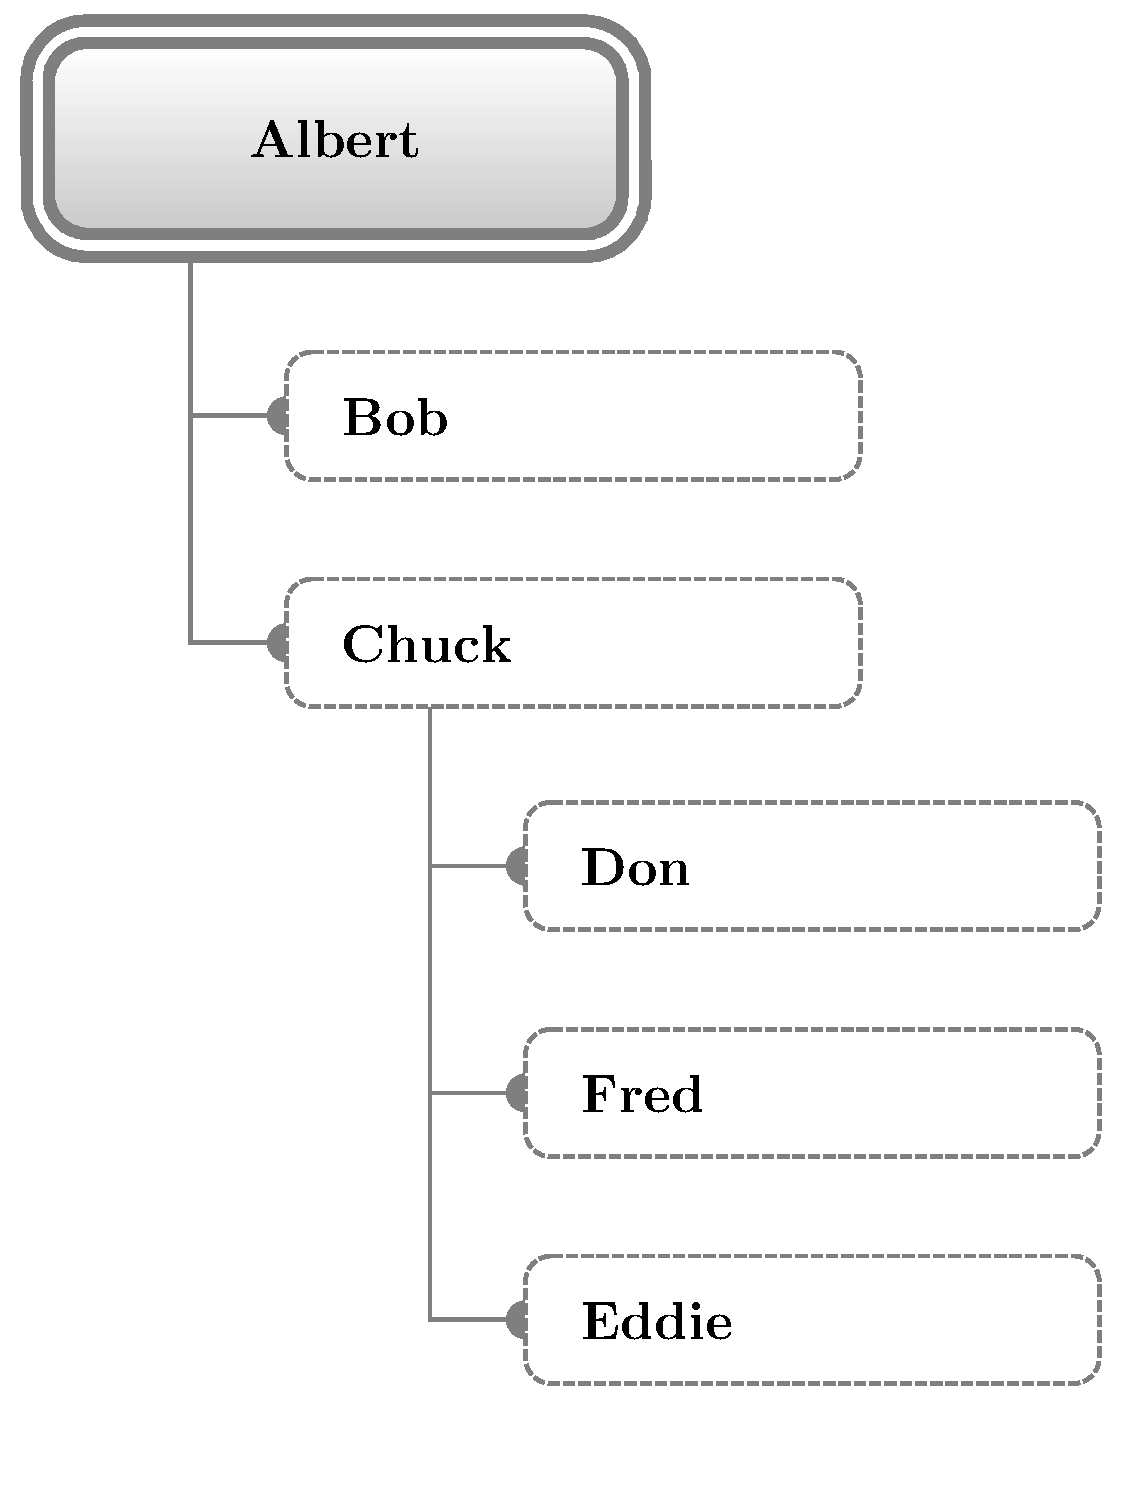
\includegraphics[width=5cm]{graphics/02-strom}
\caption{Ukázkový strom}\label{fig:stri}
\end{figure}

\begin{table}
\centering
\caption{Hranová reprezentace stromu}\label{tab:str1}
\begin{tabular}{c | c}
id & rodič \\
\hline
Albert & Albert (nebo NULL) \\
Bob & Albert \\
Chuck & Albert \\
Don & Chuck \\
Fred & Chuck \\
Eddie & Chuck
\end{tabular}
\end{table}

Vidíme, že pokud jsou hodnoty v obou sloupcích shodné nebo je hodnota ve sloupci \textit{rodič} rovna hodnotě NULL, pak je daný uzel kořenem stromu. Již letmým pohledem vidíme, že tabulka obsahuje relativně minimum dat a nedá se z ní vyčíst například, zda Chuck je levým nebo pravým potomkem Alberta. Implementace vyhledávacího stromu je tedy prakticky nemožná.

%% TODO: Obrázek stromu

\subsubsection{Cestová reprezentace}
V cestové reprezentaci je pro každý uzel popsána jeho úplná cesta napříč celým stromem. V tomto případě je nejlepší pohled na tabulku \ref{tab:str2}, která způsob reprezentace dokonale vystihuje.

\begin{table}
\centering
\caption{Cestová reprezentace stromu}\label{tab:str2}
\begin{tabular}{c | c}
id & cesta \\
\hline
Albert & /Albert \\
Bob & /Albert/Bob \\
Chuck & /Albert/Chuck \\
Don & /Albert/Chuck/Don \\
Fred & /Albert/Chuck/Fred \\
Eddie & /Albert/Chuck/Eddie
\end{tabular}
\end{table}

Na procházení takto reprezentovaného stromu se hodí operátor\upinlinecode{SQL}{!}{LIKE} z \upabbrevref{SQL}.

\subsubsection{Reprezentace vnořenými množinami}
Speciální reprezentace, která se již neřadí mezi naivní, nýbrž pokročilé. Využivá v podstatě kombinace preorder a postorder průchodů stromem, kdy se každý uzel ohodnocuje dvojicí čísel, které popisují jeho \enquote{pořadí} ve stromu. Více napoví tabulka \ref{tab:str3}.

\begin{table}
\centering
\caption{Reprezentace stromu vnořenými množinami}\label{tab:str3}
\begin{tabular}{c | c c}
id & lt & rt \\
\hline
Albert & 1 & 12 \\
Bob & 2 & 3 \\
Chuck & 4 & 11 \\
Don & 5 & 6 \\
Fred & 7 & 8 \\
Eddie & 9 & 10
\end{tabular}
\end{table}

Bystré oko čtenáře vidí, jak se strom tímto způsobem \enquote{ohodnocuje}. Hodnoty atributů \textit{lt} a \textit{rt} odhalují vlastnosti a umístění jednotlivých uzlů ve stromů.

\begin{upexample}[Dotazy na části množinově reprezentovaného stromu]
Vidíme, že kořen má zvláštní hodnotu ve sloupci \textit{lt}.

\begin{upcode}{Dotaz na kořen stromu v množinové reprezentaci}{}{SQL}
SELECT * FROM tree WHERE lt = 1;
\end{upcode}

Také listy mají poněkud unikátní vztah mezi oběma hodnotami.
\begin{upcode}{Dotaz na listy stromu v množinové reprezentaci}{}{SQL}
SELECT * FROM tree WHERE lt = rt - 1;
\end{upcode}

Velkou zbraní této reprezentace je určení podstromu určitého uzlu.
\begin{upcode}{Dotaz na podstrom stromu v množinové reprezentaci}{}{SQL}
SELECT	tree_1.id AS from_node, tree_2.id AS to_node
FROM	tree AS tree_1, tree AS tree_2
WHERE	tree_2.lt BETWEEN tree_1.lt AND tree_1.rt;
\end{upcode}
\end{upexample}


\upendoftreatise

% vytiskne seznam zkratek
\upprintabbrevlist

% tiskne seznam teorémů
\upprinttheoremlist

% vytiskne bibliografii
\upprintbibliography

% vytiskne rejstřík
%\upprintindex

\end{document}